\chapter{El Camino para Adaptar la Inteligencia Artificial en la Maquiladora}
\label{camino-adaptacion-ia-maquiladora}

\subsection{Introducción}

Hoy en día, la \textbf{Inteligencia Artificial (IA)} ya no es un lujo ni una moda pasajera; es una herramienta esencial para seguir siendo competitivo en la industria maquiladora. En lugares como \textbf{Ciudad Juárez}, donde la maquila es el mero corazón económico, adaptarse a la IA puede marcar la diferencia entre lideraar el mercado o quedarte atrás viendo cómo otros te comen el mandado. Pero, \textit{¡aguas!}, no es tan fácil como meterle otro software o cambiar una máquina. Implementar IA trae sus propios retos, y todo depende de factores como la complejidad técnica, el tiempo que te va a tomar, la lana que necesitas invertir, y qué tan listos estén tus trabajadores para aceptar el cambio y adaptarse.

Para hacerte la vida más sencilla y que no te avientes sin saber, hemos desarrollado un \textbf{Ranking de Adaptación a la IA en la Maquiladora}. Este ranking te ayuda a desglosar los factores clave, de tal manera que puedas evaluar qué tan complicado va a ser subirse al tren de la IA y qué áreas necesitan más atención.
\section{Motivo de los Proyectos de Exploración en IA para la Maquila}

La neta, meterse de lleno en la \textbf{Inteligencia Artificial (IA)} es como abrir una caja de Pandora: te enfrentas a un chorro de oportunidades, pero también a un montón de retos que, si no les entras con calma, te pueden comer. En la maquila de \textbf{Ciudad Juárez}, donde todo se mueve rápido y la competencia es feroz, la IA no solo es una moda, sino una necesidad para seguir rifando. Pero, antes de aventarnos como el Borras, necesitamos echarle coco a cómo y dónde la IA puede hacer la diferencia.

Estos proyectos que proponemos no son soluciones definitivas, ni mucho menos. Son más bien ideas para explorar el potencial de la IA, una especie de mapa del tesoro donde las X marcan las áreas clave que podrían beneficiarse de su implementación. Y ojo, porque aquí el chiste es tantear el terreno, hacer pruebas en chiquito para luego escalar en grande. O sea, estamos hablando de \textit{posibilidades}, no de certezas. La clave es ir probando, ver qué pega y ajustar sobre la marcha, como en cualquier jale de maquila.

Cuando decimos "exploración", nos referimos a meter la IA en áreas donde sabemos que podría traer buen jale, pero sin casarnos con la idea de que lo que estamos haciendo es la solución definitiva. Es como sacar un prototipo y probarlo en la línea de producción: si funciona, se escala; si no, se ajusta. Y es justo eso lo que queremos con estos proyectos: abrir la puerta a la innovación sin volarnos la barda, con un enfoque bien aterrizado en la realidad de la maquila juarense.

\subsection{Exploración y Posibles Áreas de Oportunidad}

Aquí está lo mero bueno: ¿por dónde empezamos? La respuesta corta es que hay un montón de caminos, y todos tienen el potencial de transformar la maquila de maneras que aún no alcanzamos a imaginar. Pero vámonos tranquilos. Para empezar, tenemos que identificar esas áreas clave donde la IA puede meterle nitro a los procesos, y luego irnos ajustando según lo que vayamos viendo.

Una de las primeras ideas que viene a la mente es \textbf{el control de temperatura con visión por computadora}. La temperatura en la maquila es como el ritmo cardíaco de una persona: si no la tienes bien controlada, todo se puede ir al carajo. En procesos de manufactura, un desliz en la temperatura puede significar que la calidad del producto final se venga abajo. Con IA, podríamos monitorear en tiempo real las variaciones mínimas y ajustar los procesos automáticamente antes de que haya una bronca mayor. Esto, compa, no solo te ahorra tiempo, sino también lana en mermas y reprocesos.

Otro campo que pinta bien interesante es \textbf{el análisis de datos no supervisado}. Aquí ya entramos en terreno pesado, donde la IA se pone a chambear sola, buscando patrones ocultos que ni siquiera sabíamos que existían. Imagínate que tienes un montón de datos de producción, inventarios, tiempos de entrega, y sin hacerle nada, la IA empieza a identificar qué procesos andan fallando o cómo puedes optimizar la cadena de suministro. Es como tener un compa que ve cosas que tú no ves, pero que puede cambiar las reglas del juego. Esto puede aplicarse desde el control de calidad hasta la predicción de fallas en equipos, y lo mejor es que puedes implementar estas soluciones sin necesidad de un ejército de ingenieros.

Pero no se trata solo de implementar por implementar. La clave es hacerlo bien, y aquí es donde entramos en la \textbf{unión de sistemas tradicionales, como el WMS, con LLMs (Large Language Models)} tipo ChatGPT o Gemini. Porque, si lo piensas bien, muchas de las reglas de negocio en la maquila son decisiones que toman los supervisores o el área de ventas basadas en experiencia. Con un LLM, puedes automatizar ese conocimiento y hacer que el sistema tome decisiones inteligentes sin necesidad de intervención humana cada rato. Imagínate una interfaz donde tus operarios o asesores de ventas puedan interactuar directamente con la IA para afinar el proceso de producción o ajustar la logística de distribución en tiempo real. ¡Eso es futuro!

\subsection{El Futuro de la Maquila con IA}

Así que aquí estamos, parados en la línea de salida. Estos proyectos que planteamos son apenas el primer paso de lo que podría ser una transformación total en la maquila. Pero para que funcione, necesitamos meternos de lleno en la mentalidad de exploración. No todo va a salir a la primera, y habrá cosas que tengamos que ajustar sobre la marcha. La diferencia entre las maquilas que sigan rifando y las que se queden atrás va a estar en qué tan rápido y qué tan bien adapten la IA a sus procesos.

Lo más importante, y esto no lo podemos olvidar, es que la IA no viene a reemplazar al jale humano, sino a complementarlo, a darle ese empujón extra para que todo funcione más rápido, mejor y con menos errores. Y claro, como todo en la maquila, si lo hacemos bien, nos ponemos un paso adelante de la competencia. Si no, nos quedamos viendo cómo otros se llevan el mandado. Así que no hay de otra: ¡a explorar se ha dicho!

\section{Tiempo de Desarrollo y Equipos para Proyectos de IA}

Uno de los principales retos en la maquila es el tiempo. Aquí las cosas no se pueden hacer a la ligera: hay que entregar resultados, y hay que hacerlo rápido. Sabemos que el éxito de cualquier proyecto depende en gran parte de su capacidad para cumplir con los plazos establecidos, porque en la maquila si no entregas a tiempo, pierdes clientes y oportunidades. Por eso, todos los proyectos de IA que hemos planteado tienen un tiempo de desarrollo estimado de \textbf{6 meses}, un periodo en el que buscamos probar, ajustar y entregar resultados.

Implementar IA no es algo que puedas hacer de un día para otro, pero con una planeación adecuada y un equipo sólido, es posible lograr resultados tangibles dentro de ese plazo. La clave está en utilizar un \textbf{equipo base de Data Science} bien capacitado, con roles claros y definidos, que permita avanzar de manera constante sin descuidar los detalles.

\subsection{Equipo Base de Data Science}

El equipo de Data Science para proyectos de IA en la maquila debe ser compacto, pero eficiente. Generalmente, este equipo está compuesto por los siguientes roles:

\begin{itemize}
    \item \textbf{Científico de Datos Senior}: Encargado de liderar el análisis de datos y la construcción de modelos de IA. Esta persona debe tener experiencia en proyectos de gran envergadura y conocimiento profundo en machine learning y algoritmos de optimización.
    \item \textbf{Ingeniero de Datos}: Responsable de gestionar y procesar grandes volúmenes de datos. Su trabajo es asegurarse de que los datos fluyan correctamente desde las fuentes hasta los modelos de IA, garantizando la calidad y consistencia de la información.
    \item \textbf{Desarrollador de IA}: El encargado de integrar los modelos en los sistemas de producción. Este rol es crucial para asegurar que lo que se desarrolla en el equipo de ciencia de datos se pueda aplicar de forma efectiva en la operación diaria de la maquila.
    \item \textbf{Analista de Negocios}: Su función es traducir los resultados de los modelos de IA a insights que los equipos operativos puedan entender y aplicar. También ayuda a definir los KPI y las métricas de éxito del proyecto.
    \item \textbf{Coordinador de Proyectos}: Asegura que todos los miembros del equipo estén alineados y que los plazos se cumplan. Este rol es vital para garantizar que el proyecto se mantenga en curso y se ajuste a los tiempos establecidos.
\end{itemize}

\subsection{Tabla de Sueldos del Equipo de Data Science}

A continuación, se presenta una tabla con los sueldos mensuales estimados para los diferentes roles que conforman el equipo de Data Science en la maquila. Estos salarios se ajustan a los rangos estándar del mercado para profesionales en estas áreas, y varían entre \textbf{23,000 a 42,000 MXN mensuales} dependiendo del nivel de experiencia y especialización.

\begin{table}[H]
\centering
\caption{Sueldos del Equipo de Data Science}
\resizebox{\textwidth}{!}{
\begin{tabular}{|l|c|c|}
\hline
\textbf{Rol} & \textbf{Rango Salarial (MXN/mes)} & \textbf{Descripción} \\ \hline
Científico de Datos Senior & 35,000 - 42,000 & Lidera la creación de modelos de IA y análisis avanzado de datos. \\ \hline
Ingeniero de Datos & 30,000 - 38,000 & Maneja grandes volúmenes de datos y asegura la calidad y flujo de información. \\ \hline
Desarrollador de IA & 28,000 - 35,000 & Implementa modelos de IA en sistemas de producción. \\ \hline
Analista de Negocios & 23,000 - 30,000 & Traduce los resultados de IA a estrategias de negocio. \\ \hline
Coordinador de Proyectos & 25,000 - 32,000 & Gestiona el equipo y asegura el cumplimiento de plazos y objetivos. \\ \hline
\end{tabular}}
\end{table}

\subsection{Reflexión sobre el Tiempo de Desarrollo}

Al tener un equipo de este calibre, es posible completar proyectos de IA en un lapso de 6 meses, siempre y cuando los objetivos estén bien definidos y el flujo de trabajo esté optimizado. En la maquila, donde el tiempo es dinero, contar con un equipo ágil y bien remunerado puede marcar la diferencia entre el éxito o el fracaso de una iniciativa de IA. Con la infraestructura adecuada y el talento correcto, podemos transformar áreas clave de la operación, desde la cadena de suministro hasta la gestión de calidad, en un tiempo récord.

\section{Equipo y Costos del Proyecto usando APIs LLM}

En el desarrollo de proyectos basados en \textbf{APIs de Modelos de Lenguaje (LLM)}, como los de \textit{ChatGPT} o \textit{Gemini}, es fundamental contar con un equipo capaz de implementar las soluciones técnicas, pero también con una persona que comprenda a fondo la lógica de negocio. Esta última es clave para conectar la tecnología con las necesidades operativas de la maquila y asegurar que los resultados sean tangibles y aplicables. 

El equipo ideal para un proyecto de este tipo incluye:

\begin{itemize}
    \item \textbf{2 Desarrolladores}: Su tarea principal es la integración de los LLM en los sistemas existentes y la creación de interfaces o soluciones que utilicen estos modelos para mejorar procesos específicos dentro de la maquila. 
    \item \textbf{Encargado del Proyecto}: Esta persona debe tener un profundo conocimiento de la lógica de negocio y las reglas operativas. Su función principal es traducir las necesidades del negocio en especificaciones que los desarrolladores puedan implementar usando las APIs LLM. Este rol es crítico para asegurar que el proyecto cumpla con los objetivos estratégicos de la maquila.
    \item \textbf{Uso de API de LLM}: Para estimar los costos del uso de una API LLM, se considera un rango de $10$ USD por cada 100 llamadas. Dependiendo de la escala del proyecto, el número de llamadas a la API puede variar desde miles hasta cientos de miles de interacciones por mes, afectando directamente los costos operativos.
\end{itemize}

\subsection{Costos Estimados para un Proyecto de APIs LLM}

A continuación, se presenta una tabla con los sueldos estimados para los roles clave en el proyecto, así como los costos asociados al uso de las APIs de LLM, basados en un rango estimado de llamadas a las APIs.

\begin{table}[H]
\centering
\caption{Costos del Proyecto con Uso de APIs LLM}
\resizebox{\textwidth}{!}{
\begin{tabular}{|l|c|c|}
\hline
\textbf{Rol/Componente} & \textbf{Rango Salarial/Costos (MXN/mes)} & \textbf{Descripción} \\ \hline
Desarrollador 1 & 28,000 - 37,000 & Desarrollo e integración de la API de LLM con los sistemas actuales. \\ \hline
Desarrollador 2 & 28,000 - 37,000 & Colabora en el desarrollo y optimización de las soluciones basadas en LLM. \\ \hline
Encargado del Proyecto & 35,000 - 42,000 & Responsable de la lógica de negocio, traduce las necesidades empresariales en especificaciones técnicas. \\ \hline
Uso de API de LLM (100 llamadas/mes) & \textasciitilde 200 MXN/mes & Bajo volumen de llamadas a la API, para proyectos pequeños. \\ \hline
Uso de API de LLM (10,000 llamadas/mes) & \textasciitilde 20,000 MXN/mes & Proyectos de mayor escala con interacción frecuente. \\ \hline
Uso de API de LLM (100,000 llamadas/mes) & \textasciitilde 200,000 MXN/mes & Proyectos de gran envergadura con alta demanda de procesamiento. \\ \hline
\end{tabular}}
\end{table}

\subsection{Reflexión sobre el Uso de APIs LLM}

En proyectos que utilizan APIs de LLM, la clave está en encontrar el equilibrio entre la cantidad de llamadas a la API y el impacto de los resultados. La persona encargada del proyecto debe tener una visión clara de cómo la inteligencia artificial puede agregar valor al negocio, mientras que los desarrolladores implementan estas soluciones técnicas. El \textbf{uso adecuado de APIs LLM} permite a la maquila acceder a soluciones avanzadas de IA sin necesidad de desarrollar modelos desde cero, lo que reduce el tiempo de implementación y los costos iniciales, pero es importante monitorear el uso de las API para controlar los costos operativos.


\subsection{Descripción Detallada del Ranking de complejidad}

\begin{enumerate}
    \item \textbf{Complejidad Técnica}:
    \begin{itemize}
        \item \textbf{Alto (5)}: Proyectos que requieren conocimientos avanzados y especializados en inteligencia artificial, como la implementación de \textit{redes neuronales profundas} para realizar análisis en tiempo real o sistemas de \textit{mantenimiento predictivo} que monitorean cientos de variables a la vez. En este nivel, no solo se necesitan ingenieros con experiencia en programación avanzada, sino también una infraestructura robusta que permita manejar grandes cantidades de datos. Además, este tipo de proyectos suele necesitar un equipo especializado en IA, lo que implica una fuerte inversión en talento.
        
        \item \textbf{Medio (3)}: Proyectos que requieren algo de conocimiento en programación y análisis de datos, pero no a niveles tan complejos. Por ejemplo, el uso de \textit{visión por computadora} para el control de calidad de los productos es una opción más accesible, ya que existen soluciones prefabricadas que pueden ser personalizadas para cada empresa. Aquí el equipo debe tener habilidades técnicas, pero no es necesario ser un experto en IA. La implementación es más sencilla, pero aún requiere cierta integración técnica.
        
        \item \textbf{Bajo (1)}: Soluciones listas para usarse, como las plataformas de \textit{análisis de datos} con configuraciones predefinidas. Estas herramientas permiten a las maquilas obtener información valiosa sin necesidad de contar con un equipo técnico especializado. En este caso, el esfuerzo técnico es mínimo, y muchas veces no es necesario más que conectar los sistemas existentes a la nueva herramienta. Es ideal para quienes buscan resultados rápidos sin complicaciones técnicas.
    \end{itemize}

    \item \textbf{Tiempo de Implementación}:
    \begin{itemize}
        \item \textbf{Largo (5)}: Proyectos que pueden tardar más de un año en completarse. Por ejemplo, el desarrollo de un sistema de IA que gestione toda la \textit{cadena de suministro}, desde la planificación de inventarios hasta la distribución de productos, requiere una gran cantidad de tiempo para su implementación. La razón de estos tiempos tan largos es que implican personalización y ajustes constantes para asegurar que el sistema funcione de acuerdo a las necesidades específicas de la maquila.
        
        \item \textbf{Medio (3)}: Proyectos que suelen tomar entre seis meses y un año. Este tipo de iniciativas, como la optimización de inventarios o la automatización parcial de algunos procesos, requieren tiempo para su implementación, pero no tanto como los proyectos más ambiciosos. Aquí se puede avanzar más rápido, pero aún se necesitan varios meses para integrar las soluciones, capacitar al personal y ajustar los sistemas.
        
        \item \textbf{Corto (1)}: Proyectos rápidos que se pueden completar en menos de seis meses, como la automatización de tareas administrativas o el uso de sistemas de análisis predictivo para áreas específicas de la maquila. Este tipo de soluciones permite obtener resultados inmediatos con poco tiempo de implementación, lo cual es ideal para maquilas que buscan mejoras rápidas sin detener sus operaciones durante mucho tiempo.
    \end{itemize}

    \item \textbf{Inversión Económica}:
    \begin{itemize}
        \item \textbf{Alta (5)}: Proyectos costosos que requieren una inversión significativa en tecnología, infraestructura y talento. Implementar robots industriales con IA, o crear sistemas de predicción de demanda en tiempo real para optimizar la producción, no solo requiere comprar tecnología de punta, sino también desarrollar plataformas a medida. Además, hay que tener en cuenta los costos de capacitación del personal y la adaptación de las líneas de producción a las nuevas tecnologías.
        
        \item \textbf{Media (3)}: Inversiones más accesibles, donde se puede adquirir tecnología estándar o modular que ya está disponible en el mercado, como los sistemas de \textit{mantenimiento predictivo} o los sistemas de \textit{control de calidad} que usan visión por computadora. Aquí el gasto es moderado y se puede ir implementando en fases, lo que permite distribuir el costo a lo largo del tiempo.
        
        \item \textbf{Baja (1)}: Proyectos más accesibles económicamente, como las plataformas de \textit{análisis de datos} listas para usar o el uso de asistentes virtuales para automatizar tareas sencillas. En este caso, la inversión es mínima, ya que muchas de estas herramientas se ofrecen como servicios por suscripción que no requieren grandes desembolsos iniciales, y su implementación es rápida y fácil.
    \end{itemize}

    \item \textbf{Capacitación del Personal}:
    \begin{itemize}
        \item \textbf{Alta (5)}: Proyectos que requieren una capacitación intensiva para el personal, sobre todo en casos donde la implementación de IA cambia radicalmente los procesos de la maquila. Por ejemplo, formar a los equipos en el desarrollo de inteligencia artificial, en el análisis de datos, y en la gestión de proyectos grandes que involucren IA es esencial para proyectos de gran envergadura. En estos casos, la curva de aprendizaje es alta, y los empleados tendrán que adquirir nuevas habilidades que no están presentes en la operación tradicional.
        
        \item \textbf{Media (3)}: Capacitación moderada que implica enseñar a los empleados a utilizar nuevas herramientas de IA sin necesidad de que aprendan a programar o a diseñar los sistemas. Ejemplos incluyen el entrenamiento del personal en el uso de software de control de calidad automatizado o sistemas de gestión de inventarios que utilicen IA. Aquí la curva de aprendizaje es más baja, pero el personal aún debe familiarizarse con nuevas tecnologías.
        
        \item \textbf{Baja (1)}: Proyectos que requieren una capacitación mínima para el personal, generalmente porque las herramientas son fáciles de usar y no requieren conocimientos técnicos avanzados. Herramientas como plataformas de análisis de datos o asistentes virtuales suelen ser intuitivas, por lo que el equipo puede empezar a utilizarlas casi inmediatamente, con una formación básica.
    \end{itemize}

    \item \textbf{Impacto en la Cultura Organizacional}:
    \begin{itemize}
        \item \textbf{Alto (5)}: Proyectos que implican un cambio profundo en la manera de operar y gestionar la maquila. La introducción de IA en todas las áreas, desde la producción hasta la administración, requiere una \textit{transformación digital} completa. Aquí no solo cambian los procesos, sino que también se modifica la estructura organizacional y la manera en que los empleados se relacionan con la tecnología. Este tipo de cambio suele ser retador porque exige una adaptación completa por parte de todos los miembros de la maquila.
        
        \item \textbf{Medio (3)}: Ajustes importantes en los flujos de trabajo que no cambian radicalmente la cultura, pero que sí exigen una adaptación por parte del personal. Por ejemplo, implementar automatización en áreas específicas o mejorar la gestión de inventarios con IA puede alterar algunos procesos, pero no afecta la operación global de la maquila. Aun así, requiere que los empleados ajusten su manera de trabajar y se adapten a nuevos flujos de trabajo.
        
        \item \textbf{Bajo (1)}: Cambios mínimos en la cultura organizacional, donde las herramientas de IA simplemente complementan las tareas ya existentes sin modificar de manera significativa cómo operan los empleados o la maquila en general. Un ejemplo sería la implementación de herramientas de análisis de datos que ayuden a mejorar la toma de decisiones, pero que no interfieran en el flujo normal de trabajo.
    \end{itemize}
\end{enumerate}

\subsection{Reflexión Final}

Este ranking te da un panorama claro de los retos y requisitos para implementar IA en tu maquila. No todas las empresas están en el mismo punto, y no todas tienen que seguir el mismo camino. Lo importante es saber dónde estás parado y planificar la transición de manera que puedas sacarle el mayor provecho a la IA sin exponerte a tantos riesgos.

\textbf{Adoptar IA} no es solo una cuestión de moda, es una necesidad para seguir siendo competitivo en un mundo donde la eficiencia, la precisión y la velocidad de adaptación son clave. Con una buena planificación y una implementación gradual, cualquier maquila puede aprovechar las ventajas de la IA. ¡Así que no te quedes atrás y súbete al tren de la tecnología! 

\begin{table}[htbp]
\centering
\caption{Ranking de Adaptación a la IA en la Maquiladora}
\label{tab:ranking-adaptacion}
\begin{tabularx}{\textwidth}{|X|X|c|}
\hline
\textbf{Factor} & \textbf{Descripción} & \textbf{Dificultad (1-5)} \\
\hline
\textbf{Complejidad Técnica} & Nivel de conocimiento técnico necesario para implementar IA. & \textbf{Alto (5)} \\
\hline
\textbf{Tiempo de Implementación} & Tiempo estimado para completar el proyecto de IA. & \textbf{Largo (5)} \\
\hline
\textbf{Inversión Económica} & Cantidad de recursos económicos necesarios para la implementación. & \textbf{Alta (5)} \\
\hline
\textbf{Capacitación del Personal} & Grado de entrenamiento que requiere el equipo. & \textbf{Alta (5)} \\
\hline
\textbf{Impacto Cultural} & Cambio en la cultura organizacional por la implementación de IA. & \textbf{Alto (5)} \\
\hline
\end{tabularx}
\end{table}





\section{Aplicaciones de la Inteligencia Artificial en la Maquiladora,Inyección de Plásticos: Antes y Después del Machine Learning}

\subsection{Ranking de Adaptación}

\begin{table}[h!]
\centering
\caption{Ranking de Adaptación del Proyecto 1}
\resizebox{\textwidth}{!}{
\begin{tabular}{@{}>{\bfseries}l*{5}{>{\centering\arraybackslash}p{2cm}}@{}}
\toprule
Factor & Complejidad Técnica & Tiempo de Implementación & Inversión Económica & Capacitación del Personal & Impacto en la Cultura \\ \midrule
Valor & Alto (5) & Medio (3) & Alto (5) & Medio (3) & Alto (5) \\ \bottomrule
\end{tabular}}
\end{table}
\subsection{Por qué la Industria de Inyección de Plásticos es Ideal para Machine Learning}

La industria de inyección de plásticos, con su alto nivel de automatización y la necesidad constante de mejorar la eficiencia y la calidad, es un campo ideal para la implementación de \textbf{Machine Learning (ML)}. A continuación, se detallan las principales razones por las que esta industria puede beneficiarse enormemente de la adopción de ML:

\subsubsection{1. Abundancia de Datos}

Uno de los mayores desafíos en muchas industrias es la falta de datos consistentes y de calidad. Sin embargo, la industria de inyección de plásticos produce grandes volúmenes de datos que pueden aprovecharse para entrenar modelos de ML. Desde sensores en las máquinas que recopilan información sobre temperatura, presión, y tiempos de ciclo, hasta cámaras de visión por computadora que registran imágenes de cada producto, estos datos son fundamentales para:

\begin{itemize}
    \item Monitorear el rendimiento de las máquinas.
    \item Detectar defectos en tiempo real.
    \item Predecir posibles fallas mecánicas.
\end{itemize}

La abundancia de datos proporciona el material necesario para entrenar modelos de ML con un alto grado de precisión.

\subsubsection{2. Complejidad en los Procesos de Producción}

La inyección de plásticos involucra procesos que, aunque estandarizados, son complejos y tienen múltiples variables que afectan el resultado final. Entre estos se incluyen:

\begin{itemize}
    \item Variaciones en la temperatura del molde.
    \item Presión de inyección.
    \item Tiempo de enfriamiento.
    \item Calidad del material plástico.
\end{itemize}

El control manual o basado en reglas predeterminadas puede no ser lo suficientemente flexible para manejar todas estas variables de manera eficiente. Los modelos de ML, por otro lado, pueden analizar y aprender de grandes conjuntos de datos para optimizar automáticamente estos parámetros, mejorando tanto la calidad del producto como la eficiencia del proceso.

\subsubsection{3. Mejora en el Control de Calidad}

El control de calidad es un aspecto crucial en la industria de inyección de plásticos. Con métodos tradicionales, los defectos pueden no detectarse hasta después de que se haya completado la producción, lo que puede generar costos elevados por reprocesamiento y desperdicio de material. Con Machine Learning, es posible:

\begin{itemize}
    \item Utilizar \textbf{visión por computadora} para inspeccionar cada pieza en tiempo real.
    \item Detectar defectos como burbujas, deformaciones, o grietas de manera más precisa y rápida que con la inspección manual.
    \item Mejorar el control de calidad mediante el uso de \textbf{Redes Neuronales Convolucionales (CNNs)}, que aprenden a identificar patrones complejos en los productos inyectados.
\end{itemize}

La capacidad de realizar inspecciones en tiempo real reduce significativamente los defectos y garantiza que solo los productos de alta calidad lleguen al mercado.

\subsubsection{4. Mantenimiento Predictivo}

Las máquinas de inyección de plásticos están en operación constante, y las fallas inesperadas pueden ser extremadamente costosas debido al tiempo de inactividad y la pérdida de producción. Machine Learning puede analizar los datos en tiempo real para identificar patrones que indiquen cuándo una máquina está en riesgo de falla. De esta manera, las empresas pueden:

\begin{itemize}
    \item Implementar programas de \textbf{mantenimiento predictivo}, donde las reparaciones se realicen solo cuando son necesarias, basadas en datos.
    \item Reducir el tiempo de inactividad no planificado, aumentando así la eficiencia operativa.
    \item Alargar la vida útil de las máquinas mediante la identificación temprana de problemas potenciales.
\end{itemize}

\subsubsection{5. Optimización del Flujo de Trabajo}

Además de mejorar el control de calidad y el mantenimiento, Machine Learning también puede optimizar el flujo de trabajo en una planta de inyección de plásticos. Los sistemas MES (Manufacturing Execution Systems) pueden integrarse con algoritmos de ML para analizar los datos de producción en tiempo real y hacer recomendaciones sobre:

\begin{itemize}
    \item Ajustes en la programación de producción para evitar cuellos de botella.
    \item La distribución óptima de recursos en la planta.
    \item Cambios en los parámetros de operación para maximizar la producción sin comprometer la calidad.
\end{itemize}

Esto no solo mejora la eficiencia, sino que también permite a las plantas reaccionar de manera proactiva ante cualquier interrupción en la producción.

\subsubsection{6. Reducción de Costos Operativos}

Finalmente, la implementación de Machine Learning en la industria de inyección de plásticos puede conducir a una \textbf{reducción significativa en los costos operativos}. Las mejoras en la eficiencia, el mantenimiento predictivo, y el control de calidad no solo aumentan la producción, sino que también minimizan el desperdicio de materiales y reducen los costos de energía.

En resumen, la industria de inyección de plásticos es un campo ideal para Machine Learning debido a la abundancia de datos, la complejidad de los procesos, la necesidad de un control de calidad más eficiente, y los beneficios en mantenimiento y optimización de los flujos de trabajo. Adoptar ML permite a las plantas ser más competitivas, productivas y eficientes en un mercado global cada vez más exigente.


\subsection{El Problema del Scrap en Máquinas sin Mantenimiento}

El scrap o desperdicio es uno de los problemas más costosos en la industria de inyección de plásticos. Ocurre cuando las máquinas, debido a la falta de mantenimiento adecuado, comienzan a producir piezas defectuosas que no cumplen con los estándares de calidad. Este problema es especialmente crítico porque el scrap no solo representa una pérdida directa de materiales, sino también de tiempo y recursos.

\subsubsection{Causas del Scrap por Falta de Mantenimiento}

La falta de mantenimiento adecuado en las máquinas de inyección de plásticos puede tener varias consecuencias que derivan en scrap. Algunas de las principales causas son:

\begin{itemize}
    \item \textbf{Desgaste de Componentes Críticos}: Piezas como boquillas, barriles y tornillos de las máquinas inyectoras, si no reciben mantenimiento o reemplazo oportuno, comienzan a desgastarse. Este desgaste afecta directamente la calidad del producto final.
    \item \textbf{Malos Parámetros de Inyección}: Con el tiempo, las variaciones de temperatura y presión en la máquina debido a componentes mal calibrados o desgastados pueden causar inyecciones inexactas.
    \item \textbf{Acumulación de Residuos}: Las máquinas sin limpieza regular acumulan residuos en las cavidades y canales del molde, lo que provoca defectos en las piezas.
\end{itemize}

El scrap generado por estas causas no solo afecta la eficiencia de la planta, sino que también genera costos adicionales en el reprocesamiento de material o en la pérdida total de las piezas fabricadas.

\begin{figure}[H]
\centering
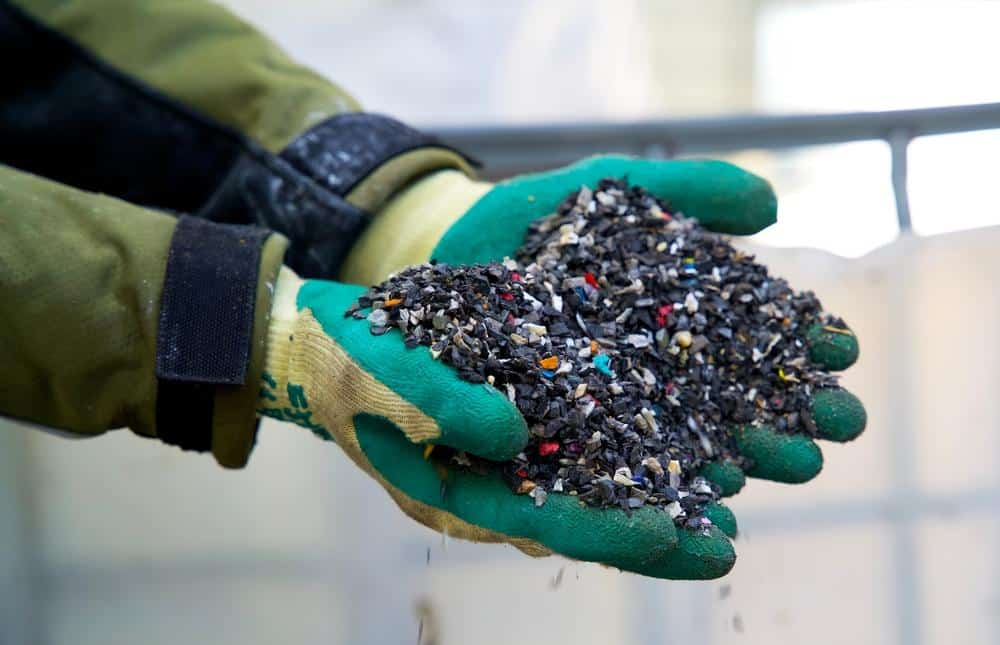
\includegraphics[width=0.7\textwidth]{img/scrap.jpg}
\caption{Ejemplo de scrap en piezas de plástico defectuosas debido a una máquina sin mantenimiento adecuado.}
\label{fig:scrap_problem}
\end{figure}



\subsection{Impacto Económico del Scrap por Falta de Mantenimiento}

El impacto económico del scrap generado por máquinas sin mantenimiento es significativo. A continuación, se describen algunos de los principales efectos:

\subsubsection{1. Pérdida de Materiales}

Cada vez que una pieza defectuosa es fabricada, se pierde material, que generalmente no puede ser reutilizado sin ser reprocesado. Esto es especialmente problemático cuando se trabaja con plásticos técnicos de alto costo, como el policarbonato o el nylon reforzado.

\subsubsection{2. Tiempo de Producción Perdido}

El tiempo dedicado a producir piezas defectuosas es tiempo perdido en la planta. Esto afecta directamente la capacidad de producción y puede generar retrasos en los envíos o incluso incumplimientos en los plazos de entrega a los clientes.

\subsubsection{3. Aumento en los Costos Operativos}

El scrap también genera un aumento en los costos operativos. Los costos de energía, mano de obra y uso de maquinaria aumentan, ya que se requiere más tiempo y recursos para producir una cantidad aceptable de piezas. Además, cuando las máquinas sin mantenimiento se detienen para reparaciones, las paradas no planificadas aumentan significativamente los costos.

\begin{figure}[H]
\centering
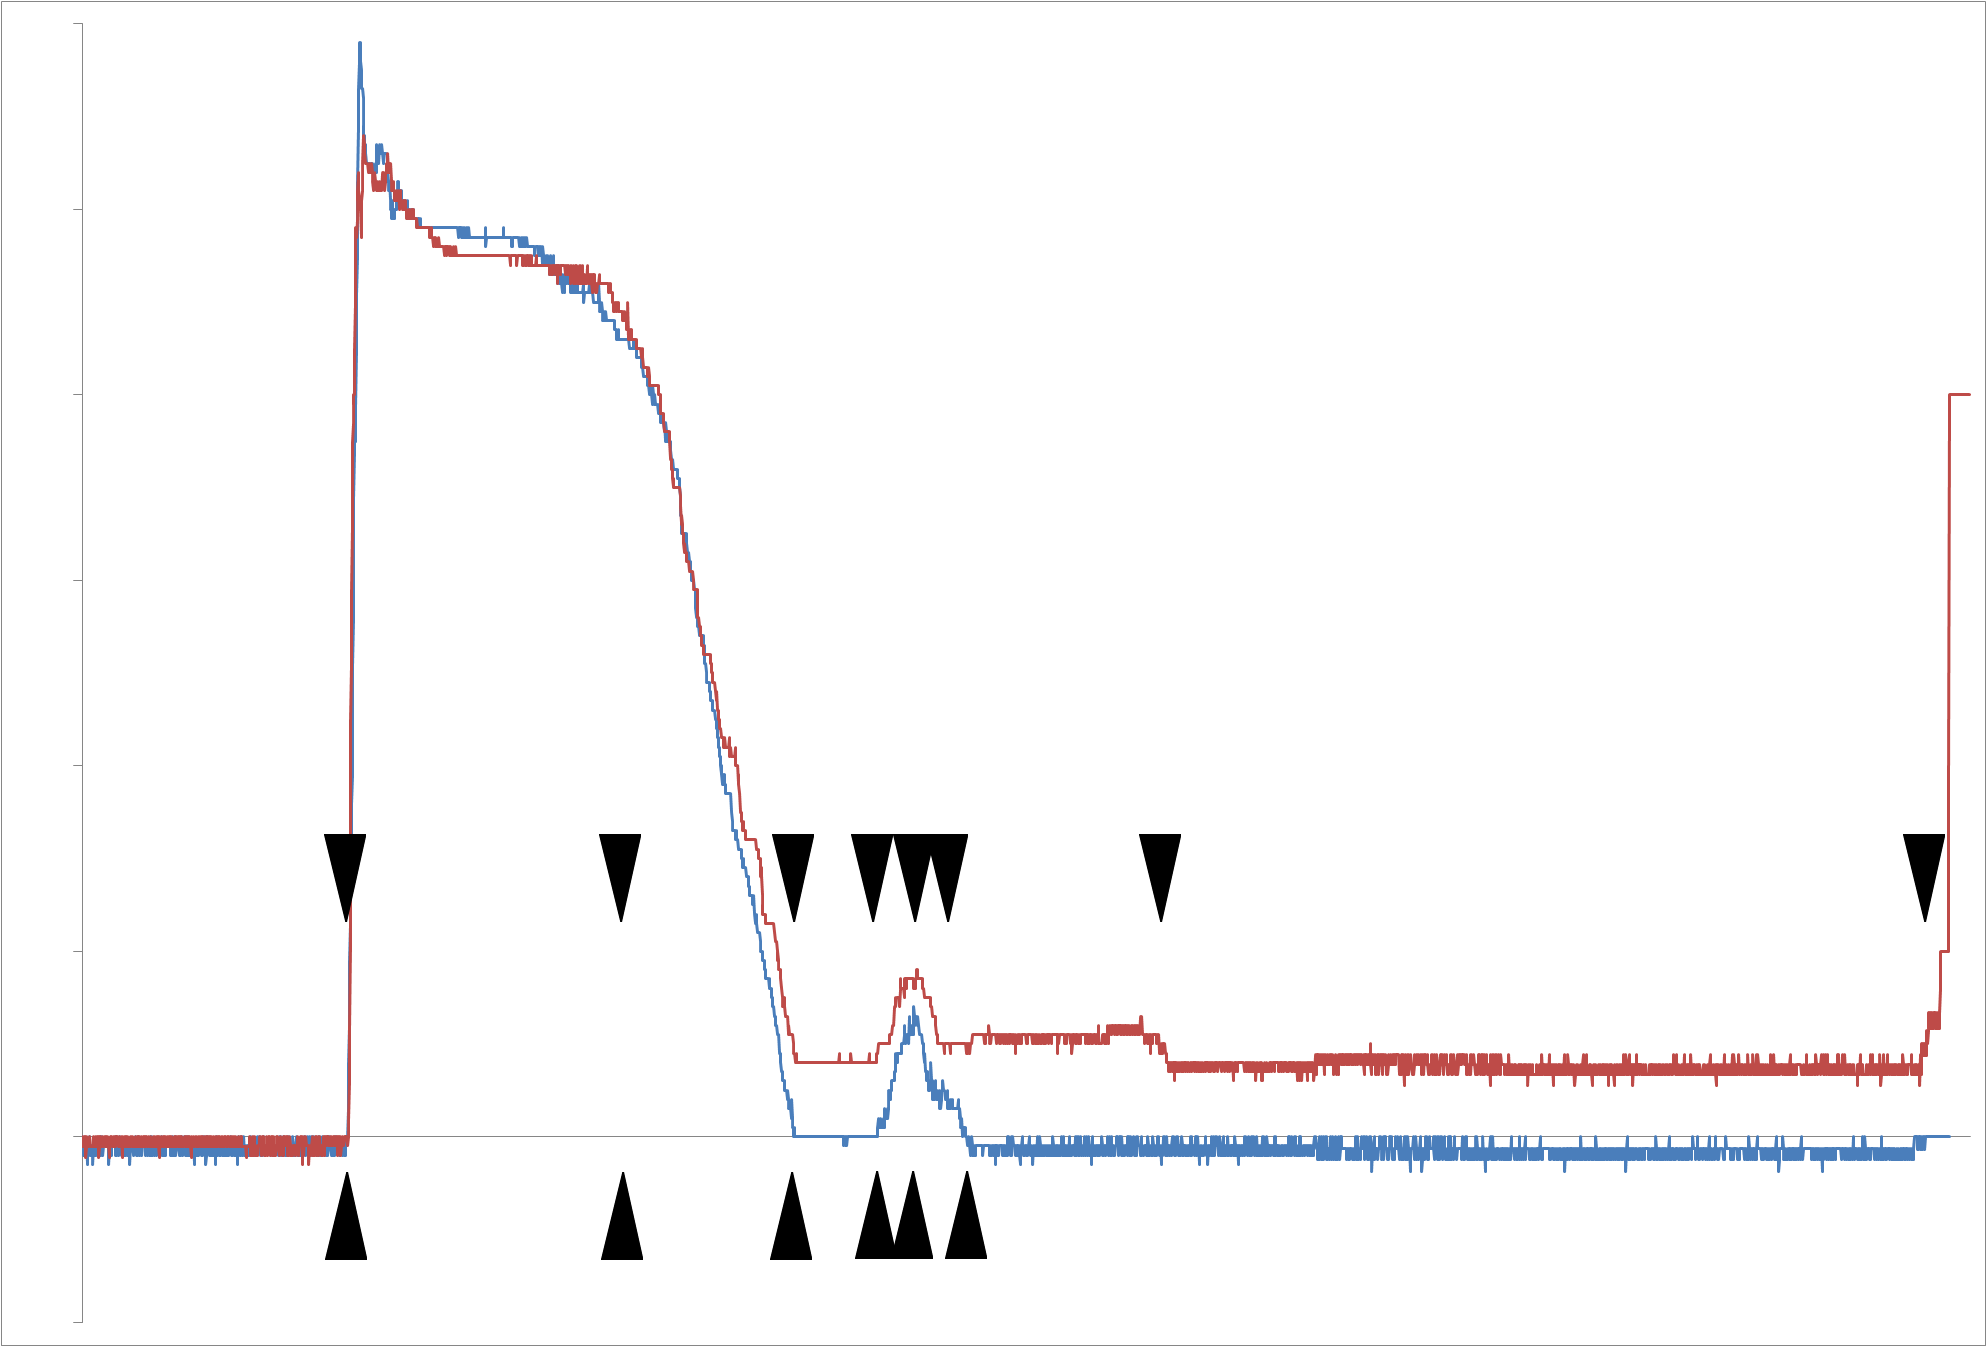
\includegraphics[width=0.7\textwidth]{img/scrap_fx.png}
\caption{Gráfico que muestra el impacto económico del scrap en una planta de inyección de plásticos.}
\label{fig:scrap_impact}
\end{figure}


\subWsection{Soluciones Basadas en Machine Learning para Reducir el Scrap}

Dado el impacto económico y operativo del scrap, una de las soluciones más prometedoras es la implementación de sistemas de Machine Learning para monitorear el estado de las máquinas y predecir cuándo se necesitarán tareas de mantenimiento. Las principales ventajas incluyen:

\begin{itemize}
    \item \textbf{Mantenimiento Predictivo}: Al monitorear los datos en tiempo real, el ML puede predecir cuándo una máquina está en riesgo de generar scrap, programando el mantenimiento necesario antes de que se produzca una gran cantidad de desperdicio.
    \item \textbf{Optimización de Parámetros de Producción}: ML puede ajustar automáticamente los parámetros de inyección, como la temperatura y la presión, para mantener la calidad de las piezas fabricadas dentro de los estándares deseados.
    \item \textbf{Reducción de Paradas No Planificadas}: Con ML, es posible anticipar fallos en las máquinas y realizar el mantenimiento en horarios planificados, evitando paradas inesperadas que generan scrap.
\end{itemize}

\begin{figure}[H]
\centering
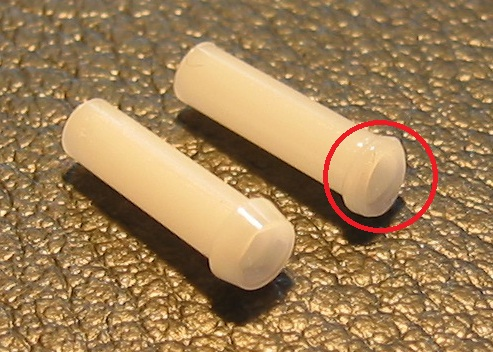
\includegraphics[width=0.7\textwidth]{img/ob_scrapt.jpg}
\caption{Detección de defectos planta de inyección de plásticos.}
\label{fig:scrap_impact}
\end{figure} 

\subsection{Control de Calidad Automatizado}

El \textbf{control de calidad automatizado} es otra aplicación clave en la maquila, utilizando IA para inspeccionar productos en la línea de producción de forma más eficiente.

\begin{table}[h!]
\centering
\caption{Tecnologías Clave en Control de Calidad Automatizado}
\resizebox{\textwidth}{!}{
\begin{tabular}{@{}>{\bfseries}l*{3}{>{\raggedright\arraybackslash}p{4cm}}@{}}
\toprule
Aplicación & Beneficios & Tecnologías Clave \\ \midrule
Control de Calidad Automatizado & Detección rápida y precisa de defectos & Cámaras de Visión por Computadora, Redes Neuronales Convolucionales, Software de Análisis de Imágenes \\ \bottomrule
\end{tabular}}
\end{table}

% Diagrama de Control de Calidad Automatizado
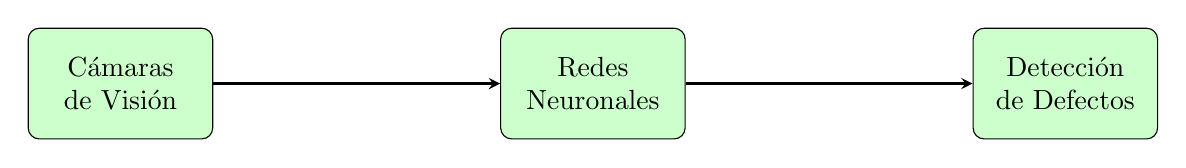
\begin{tikzpicture}[node distance=2cm]
\tikzstyle{block} = [rectangle, draw, fill=green!20, text width=6em, text centered, rounded corners, minimum height=4em]
\tikzstyle{arrow} = [thick,->,>=stealth]

\node (start) [block] {Cámaras de Visión};
\node (nn) [block, right of=start, xshift=4cm] {Redes Neuronales};
\node (quality) [block, right of=nn, xshift=4cm] {Detección de Defectos};

\draw [arrow] (start) -- (nn);
\draw [arrow] (nn) -- (quality);
\end{tikzpicture}

En el sector de la inyección de plásticos, el control de calidad automatizado es fundamental para garantizar que cada pieza cumpla con los estándares requeridos. Las cámaras de visión por computadora pueden identificar defectos como burbujas, deformaciones o imperfecciones en el moldeado.

\subsection{Optimización del Flujo de Trabajo}

La IA también puede ser utilizada para \textbf{optimizar el flujo de trabajo} en la maquila, analizando datos de producción y sugiriendo ajustes en tiempo real.

\begin{table}[h!]
\centering
\caption{Tecnologías Clave para la Optimización del Flujo de Trabajo}
\resizebox{\textwidth}{!}{
\begin{tabular}{@{}>{\bfseries}l*{3}{>{\raggedright\arraybackslash}p{4cm}}@{}}
\toprule
Aplicación & Beneficios & Tecnologías Clave \\ \midrule
Optimización del Flujo de Trabajo & Identificación de cuellos de botella, mejoras en la eficiencia & Sistemas MES, Análisis de Datos en Tiempo Real, Algoritmos de Optimización \\ \bottomrule
\end{tabular}}
\end{table}


% Diagrama de Optimización del Flujo de Trabajo
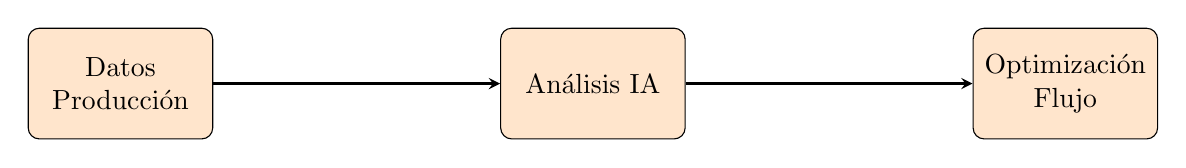
\begin{tikzpicture}[node distance=2cm]
\tikzstyle{block} = [rectangle, draw, fill=orange!20, text width=6em, text centered, rounded corners, minimum height=4em]
\tikzstyle{arrow} = [thick,->,>=stealth]

\node (start) [block] {Datos Producción};
\node (analysis) [block, right of=start, xshift=4cm] {Análisis IA};
\node (optimization) [block, right of=analysis, xshift=4cm] {Optimización Flujo};

\draw [arrow] (start) -- (analysis);
\draw [arrow] (analysis) -- (optimization);
\end{tikzpicture}

En el caso de una planta de inyección de plásticos, los sistemas MES como \textit{Siemens SIMATIC IT} pueden integrarse con la IA para detectar cuellos de botella en la producción. A través del análisis de datos en tiempo real, la planta puede ajustar la programación de los procesos, optimizando la utilización de las máquinas y reduciendo los tiempos muertos.

\subsection{Ejemplo en la Industria de Inyección de Plásticos}

En una planta de inyección de plásticos, la IA se puede aplicar de varias maneras para optimizar la operación:

\begin{enumerate}
    \item \textbf{Mantenimiento Predictivo}: Instalando sensores IoT en las máquinas de inyección, se puede monitorear el estado de las máquinas en tiempo real. La IA analiza los datos para predecir fallas, evitando costosas paradas de producción no planificadas.
    \item \textbf{Control de Calidad Automatizado}: Usando cámaras de visión por computadora y redes neuronales, la IA puede inspeccionar cada pieza de plástico en la línea de producción, detectando defectos en tiempo real.
    \item \textbf{Optimización del Flujo de Trabajo}: Con sistemas MES y análisis de datos en tiempo real, la IA puede ajustar dinámicamente el flujo de trabajo, evitando cuellos de botella y asegurando una producción continua y eficiente.
\end{enumerate}

Estas soluciones permiten que las plantas de inyección de plásticos aumenten su eficiencia, reduzcan los costos operativos y mejoren la calidad del producto final, lo que las hace más competitivas en el mercado global.

\subsection{Comparación Antes y Después del Machine Learning}

En esta sección, se muestra una comparación entre cómo se gestionaban distintos aspectos de la producción antes y después de la adopción de Machine Learning en la industria de inyección de plásticos. A través de esta comparación, se resaltan los beneficios clave que la IA ofrece.

\begin{table}[h!]
\centering
\caption{Antes y Después del Machine Learning en la Industria de Inyección de Plásticos}
\resizebox{\textwidth}{!}{
\begin{tabular}{@{}>{\bfseries}l*{2}{>{\raggedright\arraybackslash}p{6cm}}@{}}
\toprule
Proceso & Antes del Machine Learning & Después del Machine Learning \\ \midrule
Control de Calidad & Inspección manual, mayor probabilidad de error humano, identificación tardía de defectos. & Inspección automatizada en tiempo real con visión por computadora y redes neuronales, reduciendo errores y aumentando la precisión. \\ \midrule
Mantenimiento & Mantenimiento correctivo o basado en cronogramas predefinidos, alto costo por fallas inesperadas. & Mantenimiento predictivo utilizando sensores IoT y análisis de datos, anticipando fallas y reduciendo paradas no planificadas. \\ \midrule
Optimización del Flujo & Optimización reactiva basada en la experiencia del operador, identificación tardía de cuellos de botella. & Optimización proactiva del flujo de trabajo utilizando análisis de datos en tiempo real y algoritmos de Machine Learning. \\ \midrule
Eficiencia de la Producción & Dependiente de la habilidad del operador, con variabilidad en la calidad de los productos. & Eficiencia consistente y optimizada mediante el uso de algoritmos de optimización y ajustes automáticos en el flujo de trabajo. \\ \midrule
Toma de Decisiones & Basada en experiencia subjetiva, sin acceso inmediato a datos relevantes. & Toma de decisiones basada en datos, soportada por modelos predictivos que permiten mejorar la productividad y la calidad del producto. \\ \bottomrule
\end{tabular}}
}
\end{table}

\newpage

\subsection{Integración de Modelos de Lenguaje Grande (LLMs)}

Dada la creciente necesidad de optimización y automatización en la industria de inyección de plásticos, un paso inicial sencillo y efectivo para mejorar los procesos de producción es la integración de \textbf{Modelos de Lenguaje Grande (LLMs)} como primer paso, incluso si se obtiene una eficiencia inicial de solo el 61\%. 

Los LLMs pueden aportar beneficios significativos en la automatización de la comunicación interna, análisis de datos, y soporte en la toma de decisiones mediante interfaces de lenguaje natural.

\subsubsection{Eficiencia Inicial del 61\%}

Aunque la implementación de LLMs con una eficiencia inicial del 61\% puede parecer modesta, representa un avance significativo, ya que permite:

\begin{itemize}
    \item \textbf{Automatización de Consultas y Respuestas}: Los empleados pueden interactuar con el LLM para obtener respuestas rápidas sobre manuales técnicos, procedimientos de mantenimiento, y diagnósticos de fallas comunes, reduciendo el tiempo de búsqueda de información.
    \item \textbf{Soporte en la Toma de Decisiones}: El LLM puede asistir en la evaluación de datos históricos, sugiriendo posibles cursos de acción basados en patrones detectados en el historial de producción.
    \item \textbf{Mejora Gradual}: Con un punto de partida del 61\%, el sistema se puede ajustar y optimizar, alcanzando mayores niveles de eficiencia conforme se recopilan más datos y se refinan los modelos.
\end{itemize}

\subsection{Beneficios a Largo Plazo de los LLMs}

Los LLMs ofrecen una puerta de entrada para aumentar la eficiencia en la industria maquiladora, incluso con un nivel inicial de eficiencia limitado. Aquí algunos de los beneficios a largo plazo:

\begin{itemize}
    \item \textbf{Escalabilidad}: Una vez implementado, el modelo se puede entrenar con datos específicos de la planta, mejorando su precisión y alcance.
    \item \textbf{Reducción de Costos}: La automatización de tareas rutinarias y la mejora en la toma de decisiones reducirán los costos operativos a largo plazo.
    \item \textbf{Facilidad de Integración}: Los LLMs pueden integrarse fácilmente con los sistemas existentes, como ERPs y sistemas MES, para una mejor coordinación de los procesos productivos.
\end{itemize}

% Diagrama de Integración de LLMs
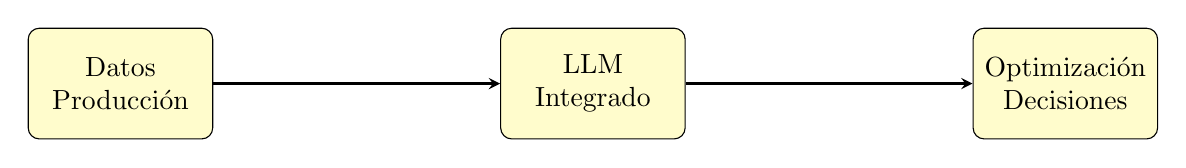
\begin{tikzpicture}[node distance=2cm]
\tikzstyle{block} = [rectangle, draw, fill=yellow!20, text width=6em, text centered, rounded corners, minimum height=4em]
\tikzstyle{arrow} = [thick,->,>=stealth]

\node (llm) [block] {LLM Integrado};
\node (data) [block, left of=llm, xshift=-4cm] {Datos Producción};
\node (output) [block, right of=llm, xshift=4cm] {Optimización Decisiones};

\draw [arrow] (data) -- (llm);
\draw [arrow] (llm) -- (output);
\end{tikzpicture}

En resumen, los LLMs pueden actuar como un primer paso accesible para automatizar y optimizar procesos en la maquiladora, con una eficiencia inicial del 61\%, que puede escalarse con el tiempo mediante ajustes y personalización del modelo.

\subsection{Conclusión}

La adopción de Machine Learning y la implementación de Modelos de Lenguaje Grande (LLMs) son pasos clave para transformar la industria de inyección de plásticos. Incluso con una eficiencia inicial del 61\%, los LLMs ofrecen una puerta de entrada hacia la automatización, la toma de decisiones basada en datos y la mejora continua, asegurando una ventaja competitiva a largo plazo.

\section{Gestión de la Cadena de Suministro con IA en la Maquiladora}

\subsection{Introducción}

La gestión eficiente de la cadena de suministro es uno de los elementos clave para el éxito de la maquiladora. El uso de \textbf{Inteligencia Artificial (IA)} en esta área permite optimizar procesos fundamentales, como la gestión de inventarios y la logística, ayudando a reducir costos, mejorar la eficiencia y aumentar la competitividad. Este capítulo presenta un análisis detallado de cómo la IA puede transformar la cadena de suministro en la industria maquiladora.

\subsubsection{Gestión de la Cadena de Suministro con IA}

El segundo proyecto se enfoca en la aplicación de IA en la gestión de la cadena de suministro. Esta solución tiene un impacto significativo en áreas clave como la \textbf{optimización de inventarios} y la \textbf{logística inteligente}, con beneficios en reducción de costos y mejora de la agilidad operativa.

\subsubsection{Ranking de Adaptación}

El siguiente ranking describe los factores clave para la implementación de IA en la gestión de la cadena de suministro:

\begin{table}[H]
\centering
\caption{Ranking de Adaptación del Proyecto 2}
\resizebox{\textwidth}{!}{
\begin{tabular}{@{}>{\bfseries}l*{5}{>{\centering\arraybackslash}p{2cm}}@{}}
\toprule
Factor & Complejidad Técnica & Tiempo de Implementación & Inversión Económica & Capacitación del Personal & Impacto en la Cultura Organizacional \\ \midrule
Valor & Medio (3) & Medio (3) & Medio (3) & Bajo (1) & Medio (3) \\ \bottomrule
\end{tabular}}
\end{table}

\subsubsection{Aplicaciones}

La IA en la gestión de la cadena de suministro tiene aplicaciones claras que ofrecen beneficios inmediatos en áreas como la optimización de inventarios y la logística. A continuación, se detallan estas aplicaciones y sus respectivos beneficios.

\subsubsection{Optimización de Inventarios}

Una de las principales preocupaciones en la cadena de suministro es el manejo eficiente de los inventarios. Con IA, las maquiladoras pueden predecir la demanda futura con mayor precisión, lo que ayuda a evitar tanto el exceso de stock (que genera costos de almacenamiento innecesarios) como la falta de stock (que puede interrumpir la producción).

\subsubsection{Beneficios}

\begin{itemize}
    \item \textbf{Reducción de costos de almacenamiento}: Mantener solo el inventario necesario, evitando excesos.
    \item \textbf{Mejora de la disponibilidad de productos}: Minimiza las interrupciones en la producción causadas por falta de insumos.
    \item \textbf{Mayor eficiencia en la cadena de suministro}: Flujo constante de materiales y productos, optimizando tiempos y recursos.
\end{itemize}

\subsubsection{Tecnologías Clave}

\begin{itemize}
    \item \textbf{Algoritmos de Predicción}: Utilizan datos históricos de demanda para predecir las necesidades futuras. Ejemplos incluyen Regresión Lineal y Redes Neuronales Recurrentes (RNNs).
    \item \textbf{Plataformas de Gestión de Inventarios}: Integran las predicciones de IA para optimizar los niveles de inventario en tiempo real.
    \item \textbf{Sensores IoT para Inventarios}: Estos sensores permiten monitorear continuamente los niveles de stock, proporcionando datos en tiempo real para decisiones más precisas.
\end{itemize}

\subsection{Logística Inteligente}

La logística en la maquiladora también puede beneficiarse considerablemente con la aplicación de IA. Los algoritmos de optimización permiten seleccionar las rutas de transporte más eficientes, programar envíos de manera óptima y realizar ajustes en tiempo real según las condiciones del mercado o la producción.

\subsubsection{Beneficios}

\begin{itemize}
    \item \textbf{Reducción de costos de transporte}: Optimización de rutas y programación de envíos más eficientes.
    \item \textbf{Mejora en los tiempos de entrega}: Capacidad para prever problemas logísticos y ajustar operaciones en tiempo real.
    \item \textbf{Mayor agilidad y capacidad de respuesta}: Respuesta rápida a cambios inesperados en la demanda o en el mercado.
\end{itemize}

\subsubsection{Tecnologías Clave}

\begin{itemize}
    \item \textbf{Algoritmos de Optimización de Rutas}: Encuentran las rutas más rápidas y económicas para el transporte de mercancías, considerando factores como el tráfico o las condiciones climáticas.
    \item \textbf{Sistemas de Gestión de Transporte (TMS)}: Utilizan IA para optimizar la planificación y ejecución del transporte, ajustando rutas y entregas en tiempo real.
    \item \textbf{Plataformas de Análisis Predictivo}: Analizan datos históricos y en tiempo real para anticipar problemas y mejorar las decisiones logísticas.
\end{itemize}

\subsubsection{Tabla Resumen de Aplicaciones y Beneficios}

A continuación, se presenta una tabla resumen de las principales aplicaciones de IA en la gestión de la cadena de suministro y sus beneficios asociados.

\begin{table}[H]
\centering
\caption{Aplicaciones de IA en la Cadena de Suministro}
\resizebox{\textwidth}{!}{
\begin{tabular}{@{}>{\bfseries}l*{3}{>{\raggedright\arraybackslash}p{4cm}}@{}}
\toprule
Aplicación & Beneficios & Tecnologías Clave \\ \midrule
Optimización de Inventarios & Reducción de costos de almacenamiento, mejora de la disponibilidad de productos, mayor eficiencia en la cadena de suministro & Algoritmos de Predicción, Plataformas de Gestión de Inventarios, Sensores IoT para Inventarios \\ \midrule
Logística Inteligente & Reducción de costos de transporte, mejora en los tiempos de entrega, mayor agilidad y capacidad de respuesta en la logística & Algoritmos de Optimización de Rutas, Sistemas de Gestión de Transporte (TMS), Plataformas de Análisis Predictivo \\ \bottomrule
\end{tabular}}}
\end{table}

\subsection{Elección de un WMS con IA en la Maquila}

En la maquila, como en cualquier industria en Ciudad Juárez, lo que más rifa es la eficiencia. Si no optimizas, te comen el mandado. Y si hablamos de optimizar, la \textbf{Inteligencia Artificial (IA)} es el compa que te ayuda a llegar al siguiente nivel. En este capítulo vamos a ver cómo elegir el mejor \textbf{Sistema de Gestión de Almacenes (WMS)} con IA según las necesidades de tu industria. Además, compararemos si es mejor comprar una solución ya hecha o armarla desde cero.

\subsubsection{Cómo Elegir un WMS con IA Según tu Área Industrial}

No todas las industrias son iguales. Cada una tiene sus necesidades y sus retos específicos, por eso necesitas un WMS que se ajuste a tu área. A continuación, te doy una guía para que elijas el más adecuado según lo que manejes en tu almacén.

\subsubsection{Industria de Manufactura}

Si estás en la manufactura, tu prioridad es controlar la materia prima y el producto terminado. Aquí necesitas un WMS que te ayude a gestionar inventarios y a coordinar a los operarios.

\textbf{Recomendación}: \textbf{Neuro+} o \textbf{Generix WMS}. Estos sistemas utilizan IA para optimizar el inventario y la disposición de los almacenes.

\subsubsection{Logística y Distribución}

En logística, lo importante es que los productos lleguen a tiempo. Necesitas un WMS con un buen TMS (Sistema de Gestión de Transporte) que optimice rutas y programe envíos.

\textbf{Recomendación}: \textbf{Oracle WMS Cloud} o \textbf{Lýseis WMS}. Estos sistemas te ayudarán a gestionar todo desde el centro de distribución hasta el destino final.

\subsubsection{Comercio Minorista}

Si estás en el comercio minorista, especialmente con una tienda en línea, necesitas mover inventarios rápidamente. La IA puede predecir la demanda y garantizar que siempre tengas el producto que los clientes buscan.

\textbf{Recomendación}: \textbf{Generix WMS}. Te permitirá predecir la demanda y preparar los pedidos de forma rápida y eficiente.

\subsubsection{Logística Internacional}

Para la logística internacional, necesitas un WMS que pueda gestionar múltiples ubicaciones, zonas horarias y trámites de aduanas.

\textbf{Recomendación}: \textbf{Oracle WMS Cloud}, ideal para empresas que operan en diversas ubicaciones y requieren una alta escalabilidad.

\subsection{Comparación: Comprar un WMS vs. Desarrollarlo Desde Cero}

¿Te compras un WMS ya hecho o lo desarrollas desde cero? Vamos a compararlos para que sepas exactamente qué implica cada opción.

\subsubsection{Comprar un WMS con IA}

Comprar un WMS ya hecho es como pedir comida a domicilio: es rápido y ya está probado, pero tiene sus limitaciones.

\textbf{Ventajas}:
\begin{itemize}
    \item Implementación rápida: En semanas ya puedes tener el sistema corriendo.
    \item Funciones probadas: Otros ya lo han utilizado con éxito.
    \item Menor riesgo técnico: No tienes que preocuparte por fallos inesperados.
    \item Actualizaciones automáticas: El proveedor se encarga de las mejoras.
\end{itemize}

\textbf{Desventajas}:
\begin{itemize}
    \item Personalización limitada: Solo puedes personalizar lo que el proveedor permite.
    \item Costos recurrentes: Las licencias y suscripciones pueden ser costosas a largo plazo.
    \item Dependencia del proveedor: Si algo falla, dependes del soporte técnico externo.
\end{itemize}

\subsubsection{Desarrollar un WMS desde Cero}

Desarrollar un WMS es como construir tu casa: lo haces a tu medida, pero requiere tiempo y dinero.

\textbf{Ventajas}:
\begin{itemize}
    \item Personalización total: Lo adaptas al 100\% a tus necesidades.
    \item Control total: Tú decides cuándo y cómo actualizar.
    \item Sin costos recurrentes: Solo pagas el desarrollo y mantenimiento.
\end{itemize}

\textbf{Desventajas}:
\begin{itemize}
    \item Tiempo de desarrollo largo: Pueden pasar meses o años antes de tener un sistema funcional.
    \item Inversión inicial alta: El desarrollo es costoso.
    \item Riesgo técnico: El desarrollo puede tener problemas no previstos.
\end{itemize}

\subsection{Tabla Comparativa: Comprar vs Desarrollar un WMS}

\begin{table}[H]
\centering
\caption{Comparación entre Comprar un WMS con IA vs Desarrollarlo desde Cero}
\resizebox{\textwidth}{!}{
\begin{tabular}{@{}lccc@{}}
\toprule
\textbf{Factor} & \textbf{Comprar un WMS} & \textbf{Desarrollar un WMS desde Cero} \\ \midrule
\textbf{Tiempo de Implementación} & Rápido (Semanas a meses) & Lento (Meses a años) \\ 
\textbf{Costos Iniciales} & Moderados (Licencias y suscripciones) & Altos (Desarrollo interno) \\ 
\textbf{Costos Recurrentes} & Altos (Suscripciones, mantenimiento) & Bajos (Solo mantenimiento interno) \\ 
\textbf{Personalización} & Limitada (Lo que permita el software) & Alta (Totalmente a medida) \\ 
\textbf{Riesgos Técnicos} & Bajos (Producto probado) & Altos (Posibles fallos en desarrollo) \\ 
\bottomrule
\end{tabular}
}
\end{table}

\subsection{Conclusión}

Ya tienes todo lo que necesitas para tomar una buena decisión sobre qué WMS con IA elegir y si es mejor comprarlo o desarrollarlo desde cero. En Ciudad Juárez, donde la maquila no se detiene, es crucial tomar la decisión correcta para optimizar tus operaciones y no quedarte atrás. Comprar un WMS es más rápido y seguro, pero si tienes tiempo y presupuesto, desarrollar uno a medida puede ser la mejor opción para tener todo bajo control y optimizado al máximo. ¡Tú decides!
\section{Integración de LLMs y WMS: La Clave para una Automatización Inteligente}

\subsubsection{Introducción}

La integración de \textbf{Modelos de Lenguaje de Gran Tamaño (LLMs)} y \textbf{Sistemas de Gestión de Almacenes (WMS)} puede ser un gran avance en la automatización inteligente de las decisiones empresariales. Estos modelos permiten gestionar las reglas de negocio de manera eficiente a través de interfaces de usuario o mediante el uso de asesores de ventas virtuales, proporcionando a las empresas flexibilidad y escalabilidad en su cadena de suministro.

Este capítulo explora cómo unir WMS con LLMs para mejorar la eficiencia en la toma de decisiones, utilizando las capacidades de IA para procesar lenguaje natural, simplificar procesos logísticos y mejorar la experiencia del cliente.

\subsection{La Clave: Unir Reglas de Negocio con LLMs}

Las reglas de negocio en los almacenes son vitales para garantizar que el inventario se gestione de manera eficiente, optimizando los tiempos de entrega y minimizando los costos. Con los LLMs, estas reglas pueden integrarse directamente en un sistema de IA que permita:

\begin{itemize}
    \item **Procesar consultas de los operadores o asesores de ventas virtuales**: Los LLMs pueden recibir información de los operadores de almacén o del personal de ventas y generar recomendaciones sobre gestión de inventarios o pedidos.
    \item **Automatizar la toma de decisiones**: Al vincular un LLM a un WMS, es posible automatizar las reglas de negocio, como la optimización de rutas de entrega o la gestión de inventarios en tiempo real.
    \item **Simplificar el flujo de trabajo mediante una interfaz de usuario**: Una interfaz de ventas o asesor virtual puede proporcionar respuestas rápidas a los clientes o al personal de ventas, optimizando las operaciones de manera proactiva y ágil.
\end{itemize}

\subsection{Análisis de Costos y Exactitud en la Integración de LLM y WMS}

La integración de un LLM con un WMS puede implicar costos variables según la escala de las operaciones y el nivel de personalización requerido. A continuación, presentamos una comparación de dos enfoques:

\begin{table}[H]
\centering
\caption{Comparación de Costos y Resultados: LLM mediante API en un WMS vs. Equipo Interno de Ciencia de Datos}
\resizebox{\textwidth}{!}{
\begin{tabular}{@{}>{\bfseries}l>{\raggedright\arraybackslash}p{5cm}>{\raggedright\arraybackslash}p{5cm}>{\raggedright\arraybackslash}p{5cm}@{}}
\toprule
\textbf{Parámetro} & \textbf{LLM mediante API en WMS} & \textbf{Equipo Interno de Ciencia de Datos} \\ \midrule
\textbf{Costo (5 meses)} & \$10 USD por 100 llamadas a la API & \$10,000 USD para contratar y mantener al equipo de IA \\
\textbf{Exactitud en 5 meses} & 63\% & Entre 76\% y 87\% \\
\textbf{Tiempo de Implementación} & Inmediato & 5 meses (estimado) \\
\textbf{Escalabilidad} & Alta (nuevas llamadas a la API son fáciles de integrar) & Media (requiere ajustar el modelo continuamente) \\
\textbf{Personalización de reglas de negocio} & Limitada (basada en modelos preentrenados) & Alta (el equipo puede adaptar las reglas según las necesidades específicas) \\ \bottomrule
\end{tabular}}
\end{table}

En este caso, la integración de LLM mediante API ofrece una implementación rápida y económica, pero con limitaciones en cuanto a la personalización de reglas de negocio. Por otro lado, un equipo de IA interno puede desarrollar modelos más precisos y adaptados al contexto específico del almacén, lo cual se refleja en una mayor exactitud (entre 76\% y 87\%) y una mayor flexibilidad en la personalización de las reglas.

\subsection{Diagrama de Flujo de Integración de LLM y WMS}

El siguiente diagrama muestra el flujo de integración de un LLM con un WMS, destacando cómo las reglas de negocio se pueden procesar a través de una interfaz de ventas o un asesor virtual.

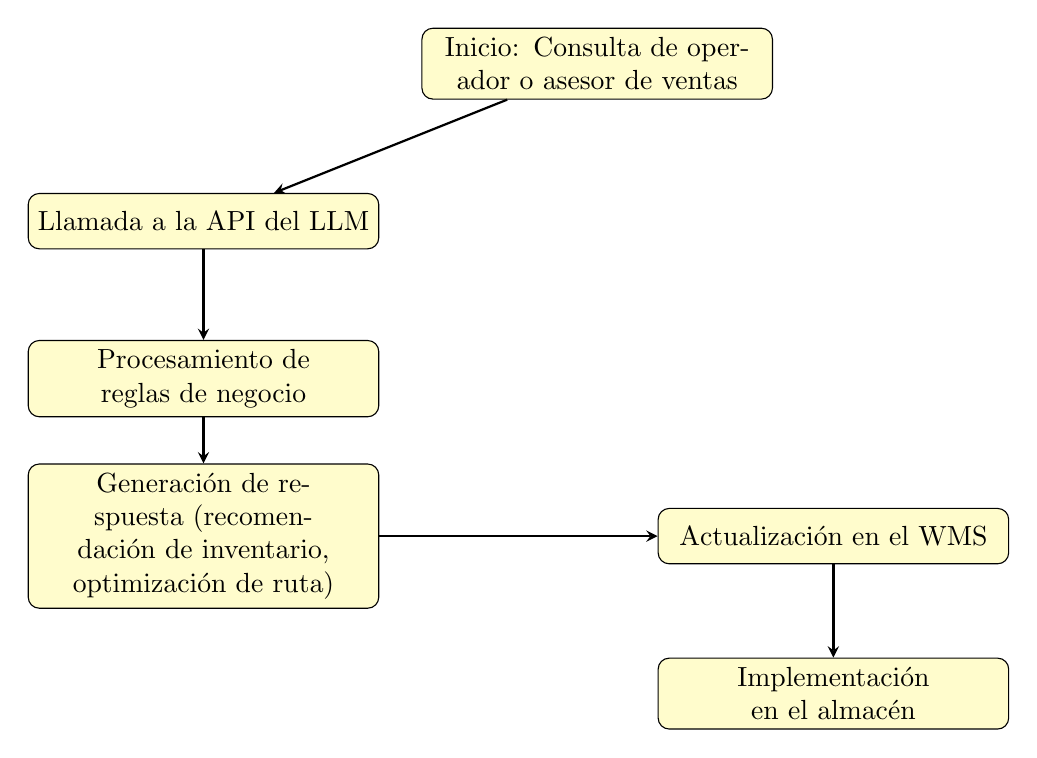
\begin{tikzpicture}[node distance=2cm, auto]
% Styles
\tikzstyle{block} = [rectangle, draw, fill=yellow!20, text centered, rounded corners, minimum height=2em, text width=12em]
\tikzstyle{arrow} = [thick,->,>=stealth]

% Nodes
\node (start) [block] {Inicio: Consulta de operador o asesor de ventas};
\node (api) [block, below of=start, xshift=-5cm] {Llamada a la API del LLM};
\node (rules) [block, below of=api] {Procesamiento de reglas de negocio};
\node (response) [block, below of=rules] {Generación de respuesta (recomendación de inventario, optimización de ruta)};
\node (wms) [block, right of=response, xshift=6cm] {Actualización en el WMS};
\node (final) [block, below of=wms] {Implementación en el almacén};

% Arrows
\draw [arrow] (start) -- (api);
\draw [arrow] (api) -- (rules);
\draw [arrow] (rules) -- (response);
\draw [arrow] (response) -- (wms);
\draw [arrow] (wms) -- (final);
\end{tikzpicture}

\subsection{Beneficios de Integrar LLM con WMS}

La integración de un LLM con un WMS puede traer una serie de beneficios operativos importantes:

\begin{itemize}
    \item **Automatización de reglas de negocio**: Los operadores o asesores virtuales pueden interactuar con el sistema mediante una interfaz que procesa reglas de negocio específicas, como la gestión de inventarios, reabastecimiento y optimización de rutas.
    \item **Mejora en la precisión de las decisiones**: A través del análisis de datos históricos y en tiempo real, el LLM puede mejorar la precisión de las decisiones operativas en el almacén.
    \item **Escalabilidad**: La implementación de un LLM permite escalar operaciones rápidamente sin necesidad de ampliar de manera significativa el equipo de trabajo.
\end{itemize}

\subsection{Evaluación Comparativa: Integración de LLM en WMS a 5 Meses}

A continuación se presenta una tabla comparativa que evalúa los resultados obtenidos al integrar un LLM con un WMS a lo largo de 5 meses, comparado con la contratación de un equipo interno de IA.

\begin{table}[H]
\centering
\caption{Evaluación de Resultados a 5 Meses: Integración de LLM en WMS vs. Equipo Interno de IA}
\resizebox{\textwidth}{!}{
\begin{tabular}{@{}>{\bfseries}l>{\raggedright\arraybackslash}p{5cm}>{\raggedright\arraybackslash}p{5cm}>{\raggedright\arraybackslash}p{5cm}@{}}
\toprule
\textbf{Parámetro} & \textbf{LLM en WMS (5 meses)} & \textbf{Equipo Interno de IA (5 meses)} \\ \midrule
Costo Acumulado & \$50 USD (500 llamadas) & \$10,000 USD (salarios y herramientas) \\
Exactitud & 63\% & Entre 76\% y 87\% \\
Personalización & Limitada (dependencia de la API) & Alta (modelos ajustados a las reglas de negocio específicas) \\
Impacto en el negocio & Resultados rápidos, útiles para prototipos y pruebas & Alta precisión, ideal para entornos de producción \\ \bottomrule
\end{tabular}}
\end{table}

\subsection{Conclusión}

Unir un LLM con un WMS ofrece una solución eficiente para automatizar y mejorar las decisiones operativas en el almacén. Aunque la exactitud y personalización del uso de LLM mediante API puede ser menor en comparación con un equipo de IA interno, el costo y la rapidez de implementación lo hacen una opción atractiva para empresas que buscan resultados inmediatos. Además, esta integración proporciona una base sólida para futuras mejoras, como el desarrollo de interfaces de ventas automatizadas que ayuden a gestionar reglas de negocio en tiempo real.

\begin{figure}[H]
\centering
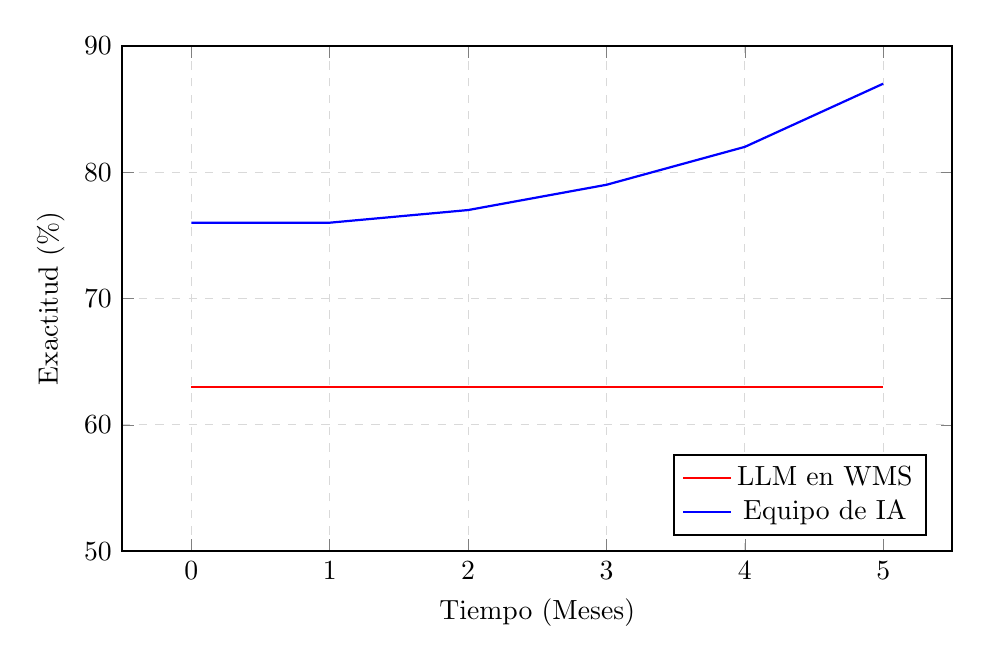
\begin{tikzpicture}
    \begin{axis}[
        width=\textwidth,
        height=8cm,
        grid=both,
        xlabel={Tiempo (Meses)},
        ylabel={Exactitud (\%)},
        legend pos=south east,
        ymin=50, ymax=90,
        grid style={dashed, gray!30},
        xtick distance=1,
        ytick distance=10,
        thick
    ]
    \addplot[color=red, thick] coordinates {
        (0, 63) (1, 63) (2, 63) (3, 63) (4, 63) (5, 63)
    };
    \addplot[color=blue, thick] coordinates {
        (0, 76) (1, 76) (2, 77) (3, 79) (4, 82) (5, 87)
    };
    \legend{LLM en WMS, Equipo de IA}
    \end{axis}
\end{tikzpicture}
\caption{Comparación de Exactitud a lo largo del Tiempo: LLM en WMS vs. Equipo Interno de IA}
\end{figure}

\section{Nuevas Áreas de Aplicación de la IA en la Industria Farmacéutica}

\subsection{Introducción}

La Inteligencia Artificial (IA) está revolucionando la industria farmacéutica, especialmente en la gestión de materias primas y el control de procesos. Más allá de los enfoques tradicionales como los sistemas de gestión de inventarios, la IA ofrece oportunidades innovadoras en áreas como el control de temperatura y el análisis de datos no supervisado. Estas tecnologías no solo permiten la optimización de recursos, sino que también mejoran la calidad y la seguridad de los productos farmacéuticos.

\subsection{Aplicaciones del Aprendizaje No Supervisado en la Industria Farmacéutica}

El aprendizaje no supervisado es una rama de la IA que se enfoca en encontrar patrones en datos sin la necesidad de etiquetas o supervisión humana. En la industria farmacéutica, el aprendizaje no supervisado puede aplicarse para detectar anomalías en la calidad de las materias primas, optimizar el control de procesos y analizar grandes volúmenes de datos.

\subsubsection{1. Detección de Anomalías en Materias Primas}

El control de calidad de las materias primas es un desafío constante en la industria farmacéutica. Con algoritmos de clustering no supervisados, como \textit{k-means} o redes neuronales autoorganizadas (SOM), es posible identificar patrones anómalos en los lotes de materias primas que podrían pasar desapercibidos con técnicas tradicionales.

\textbf{Beneficios}:
\begin{itemize}
    \item Mejora en la detección temprana de defectos o contaminación.
    \item Reducción de riesgos en la cadena de producción.
    \item Optimización del control de calidad mediante análisis automatizados.
\end{itemize}

\textbf{Tecnologías Clave}:
\begin{itemize}
    \item \textit{k-means clustering}: Agrupa las muestras en base a similitudes, permitiendo identificar grupos anómalos.
    \item \textit{Autoencoders}: Redes neuronales que identifican patrones no típicos basándose en la compresión de datos.
    \item \textit{Análisis de Componentes Principales (PCA)}: Permite reducir la dimensionalidad de los datos para detectar outliers.
\end{itemize}

\subsubsection{2. Optimización del Proceso de Fabricación}

El aprendizaje no supervisado también puede optimizar los procesos de fabricación farmacéutica mediante el análisis de datos de sensores y máquinas que controlan variables clave, como la temperatura, la presión o la humedad. La IA puede identificar combinaciones óptimas de variables para mejorar la eficiencia y reducir el consumo de energía.

\textbf{Beneficios}:
\begin{itemize}
    \item Aumento de la eficiencia de la producción.
    \item Reducción de costos energéticos.
    \item Mejora en la consistencia y calidad del producto final.
\end{itemize}

\textbf{Tecnologías Clave}:
\begin{itemize}
    \item \textit{Mapas Autoorganizados (SOM)}: Utilizados para monitorear y ajustar los parámetros de fabricación en tiempo real.
    \item \textit{Algoritmos de clustering jerárquico}: Para descubrir correlaciones entre las variables de control de proceso.
\end{itemize}

\subsection{Control de Temperatura Inteligente con IA}

El control preciso de la temperatura es esencial en la industria farmacéutica, especialmente en la fabricación y almacenamiento de medicamentos sensibles. La IA, en combinación con sistemas de monitoreo de temperatura, puede proporcionar ajustes automáticos en tiempo real, asegurando que los productos se mantengan en un rango óptimo.

\subsubsection{1. Monitoreo Predictivo de Temperatura}

Utilizando algoritmos de predicción basados en IA, es posible anticipar cambios en la temperatura dentro de los sistemas de almacenamiento o durante el transporte, lo que permite realizar ajustes antes de que los parámetros se desvíen fuera de los rangos aceptables.

\textbf{Beneficios}:
\begin{itemize}
    \item Reducción de pérdidas de productos por condiciones inadecuadas de temperatura.
    \item Mejora en la trazabilidad y seguridad del producto.
    \item Respuesta más rápida ante anomalías en las condiciones de almacenamiento.
\end{itemize}

\textbf{Tecnologías Clave}:
\begin{itemize}
    \item \textit{Redes Neuronales Recurrentes (RNN)}: Para predecir fluctuaciones de temperatura basadas en datos históricos.
    \item \textit{Modelos de Predicción Basados en Series Temporales}: Para identificar patrones de comportamiento térmico y prevenir desviaciones.
\end{itemize}

\subsubsection{2. Gestión de Almacenes Inteligentes Basada en Temperatura}

La IA también puede mejorar la disposición de productos farmacéuticos en almacenes, ubicándolos estratégicamente según sus necesidades específicas de temperatura. Esto es particularmente útil para productos que deben mantenerse en condiciones de frío o ambientes controlados.

\textbf{Beneficios}:
\begin{itemize}
    \item Optimización del uso de energía en sistemas de refrigeración.
    \item Mejora en la seguridad del almacenamiento de productos termolábiles.
    \item Reducción de desperdicios por caducidad temprana o deterioro por exposición térmica.
\end{itemize}

\textbf{Tecnologías Clave}:
\begin{itemize}
    \item \textit{Sensores IoT Integrados con IA}: Para monitorear en tiempo real la distribución de temperatura en los almacenes.
    \item \textit{Algoritmos de Optimización}: Para mejorar la disposición física de los productos y minimizar la variabilidad térmica.
\end{itemize}

\subsection{Análisis de Datos No Supervisado para la Seguridad de Medicamentos}

La IA no supervisada también puede ayudar en la farmacovigilancia, detectando patrones inusuales en los reportes de efectos adversos. El análisis de grandes volúmenes de datos sobre reacciones adversas puede identificar grupos de riesgo o correlaciones no evidentes entre los efectos secundarios y ciertos tipos de medicamentos o pacientes.

\textbf{Beneficios}:
\begin{itemize}
    \item Detección más rápida de riesgos para la seguridad de medicamentos.
    \item Reducción de riesgos asociados a reacciones adversas graves.
    \item Mejora en la toma de decisiones para la regulación y autorización de fármacos.
\end{itemize}

\textbf{Tecnologías Clave}:
\begin{itemize}
    \item \textit{Algoritmos de Clustering}: Para agrupar reportes similares de efectos adversos.
    \item \textit{Modelos de Análisis de Redes}: Para identificar relaciones entre los medicamentos y los grupos de pacientes.
\end{itemize}

\subsection{Conclusión}

El uso de IA, especialmente el aprendizaje no supervisado, ofrece un gran potencial para optimizar la gestión de materias primas y el control de procesos en la industria farmacéutica. Desde el monitoreo predictivo de la temperatura hasta la detección de anomalías en las materias primas, estas tecnologías permiten una mejora significativa en la eficiencia, calidad y seguridad del sector, manteniendo siempre la precisión que exige la industria.

\section{Comparación de Resultados: Antes y Después de la Implementación de IA}

\subsection{Control de Calidad de Materias Primas}

El siguiente cuadro muestra la diferencia en el control de calidad de materias primas antes y después de implementar técnicas de IA no supervisadas para la detección de anomalías.

\begin{table}[H]
\centering
\caption{Comparación de Control de Calidad de Materias Primas (Antes y Después de IA)}
\resizebox{\textwidth}{!}{
\begin{tabular}{@{}lcc@{}}
\toprule
\textbf{Aspecto} & \textbf{Antes de Implementar IA} & \textbf{Después de Implementar IA} \\ \midrule
Tasa de detección de defectos & Baja, basada en inspección manual & Alta, con detección automatizada por IA \\
Tiempo de detección de anomalías & Lento, inspección manual lote por lote & Rápido, análisis en tiempo real con clustering \\
Consistencia en la calidad & Variable debido a errores humanos & Alta consistencia gracias a IA automatizada \\
Costos de inspección & Altos debido al trabajo manual intensivo & Reducción significativa de costos \\ \bottomrule
\end{tabular}}
\end{table}

\subsection{Control de Temperatura en Almacenamiento}

La siguiente tabla compara el control de temperatura en almacenes farmacéuticos antes y después de la implementación de IA para el monitoreo y ajuste predictivo.

\begin{table}[H]
\centering
\caption{Comparación del Control de Temperatura (Antes y Después de IA)}
\resizebox{\textwidth}{!}{
\begin{tabular}{@{}lcc@{}}
\toprule
\textbf{Aspecto} & \textbf{Antes de Implementar IA} & \textbf{Después de Implementar IA} \\ \midrule
Monitoreo de temperatura & Manual o reactivo ante problemas & Predicción y ajuste en tiempo real con IA \\
Tiempo de respuesta ante desviaciones & Lento, con posibles daños a los productos & Inmediato, previniendo riesgos de deterioro \\
Costos de energía & Altos por ineficiencia en la refrigeración & Reducción de costos por optimización energética \\
Pérdida de productos & Alta por fallas en el control de temperatura & Significativamente reducida gracias al monitoreo predictivo \\ \bottomrule
\end{tabular}}
\end{table}

\subsection{Diagrama: Proceso de Implementación de IA en Control de Materias Primas y Temperatura}

A continuación se presenta un diagrama de flujo que describe el proceso de implementación de IA en la detección de anomalías en materias primas y en el control de temperatura en almacenes.

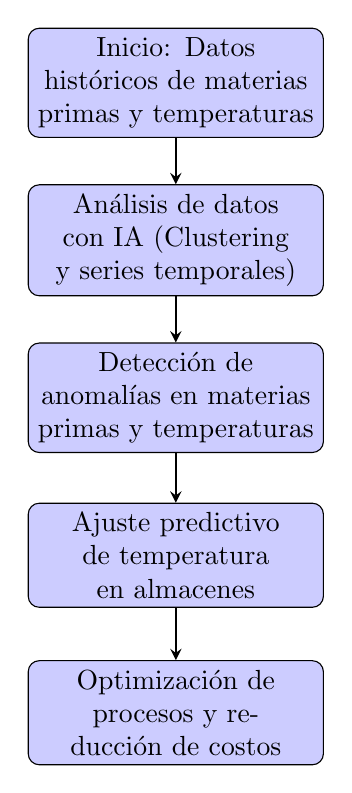
\begin{tikzpicture}[node distance=2cm, auto]
% Styles
\tikzstyle{block} = [rectangle, draw, fill=blue!20, text centered, rounded corners, minimum height=2em, text width=10em]
\tikzstyle{arrow} = [thick,->,>=stealth]

% Nodes
\node (start) [block] {Inicio: Datos históricos de materias primas y temperaturas};
\node (analyze) [block, below of=start] {Análisis de datos con IA (Clustering y series temporales)};
\node (detect) [block, below of=analyze] {Detección de anomalías en materias primas y temperaturas};
\node (adjust) [block, below of=detect] {Ajuste predictivo de temperatura en almacenes};
\node (optimize) [block, below of=adjust] {Optimización de procesos y reducción de costos};

% Arrows
\draw [arrow] (start) -- (analyze);
\draw [arrow] (analyze) -- (detect);
\draw [arrow] (detect) -- (adjust);
\draw [arrow] (adjust) -- (optimize);
\end{tikzpicture}


\section{El Potencial de los Modelos de Lenguaje en Nuevos Proyectos de IA}

La Inteligencia Artificial (IA) ha dado pasos gigantescos en los últimos años, y los \textbf{Modelos de Lenguaje de Gran Escala (LLMs)}, como \textit{ChatGPT} y \textit{Gemini}, han cambiado la forma en que las industrias piensan sobre la automatización y el procesamiento de datos. A diferencia de las aplicaciones tradicionales de IA que requerían el desarrollo de modelos específicos para cada tarea, los LLMs ofrecen una solución flexible y accesible, permitiendo el acceso a capacidades avanzadas de procesamiento del lenguaje a través de \textbf{APIs}.

Con el uso de APIs de LLMs, las empresas pueden integrar funcionalidades inteligentes en sus operaciones de manera rápida y eficiente. Esto abre una nueva era de \textbf{oportunidades de IA}, donde las maquiladoras y otras industrias pueden experimentar con soluciones que antes estaban fuera de su alcance debido a la complejidad técnica o los altos costos de desarrollo. La versatilidad de los LLMs permite utilizarlos en una amplia gama de aplicaciones, desde la automatización de procesos hasta la creación de sistemas inteligentes de recomendación, análisis de datos, e incluso asesoría virtual en tiempo real.

\subsection{Nuevas Áreas de Oportunidad en la Maquiladora con LLMs}

En la maquila, donde la eficiencia y la velocidad de adaptación son fundamentales para mantenerse competitivo, los LLMs ofrecen nuevas áreas de oportunidad que permiten escalar las operaciones sin necesidad de una gran inversión en infraestructura de IA. Aquí algunos ejemplos clave:

\begin{itemize}
    \item \textbf{Automatización del Servicio al Cliente}: Los LLMs permiten desarrollar \textit{asistentes virtuales} capaces de entender y responder preguntas complejas en diferentes idiomas, proporcionando soporte técnico o de producto de manera más rápida y eficiente. Esto ayuda a reducir los tiempos de espera y mejora la experiencia del cliente.
    
    \item \textbf{Optimización de Procesos Administrativos}: Las APIs de LLM pueden integrarse en sistemas de gestión empresarial para automatizar tareas administrativas, como la generación de reportes, procesamiento de órdenes, y manejo de inventarios. Esto libera a los empleados de tareas repetitivas, permitiendo enfocarse en actividades de mayor valor.
    
    \item \textbf{Análisis Predictivo y Toma de Decisiones}: Utilizando LLMs, las empresas pueden acceder a análisis avanzados en tiempo real, utilizando datos históricos y actuales para prever tendencias y tomar decisiones estratégicas. En combinación con datos no estructurados (como correos electrónicos o documentos), los LLMs pueden proporcionar insights valiosos para la planificación de la producción o la logística.
    
    \item \textbf{Asesores de Ventas Inteligentes}: Los LLMs pueden ser empleados para crear sistemas de recomendación personalizados, donde un \textit{asesor virtual} sugiera productos o soluciones basados en las interacciones con el cliente, ajustándose a las reglas de negocio predefinidas y optimizando las oportunidades de ventas.
    
    \item \textbf{Gestión del Conocimiento}: En lugar de recurrir a múltiples bases de datos o documentos dispersos, los LLMs permiten acceder a información relevante de manera rápida y sencilla, respondiendo preguntas sobre la operación de la maquila o resolviendo dudas técnicas en tiempo real. Esto es especialmente útil en áreas donde la capacitación del personal es constante y las actualizaciones de procesos son frecuentes.
\end{itemize}

\subsection{El Papel de las APIs en la Nueva Generación de Proyectos de IA}

El uso de \textbf{APIs de LLMs} representa un cambio en la forma en que las empresas acceden a la inteligencia artificial. Tradicionalmente, desarrollar una solución de IA requería meses de trabajo, recopilación de datos y un equipo altamente especializado en ciencia de datos y desarrollo de software. Hoy en día, gracias a las APIs, las empresas pueden integrar capacidades de IA avanzadas en sus operaciones en cuestión de semanas o incluso días. 

\subsection{Ventajas del Uso de APIs de LLMs}
\begin{itemize}
    \item \textbf{Acceso Inmediato a la IA}: Las APIs proporcionan acceso a modelos de lenguaje ya entrenados, eliminando la necesidad de desarrollar modelos propios desde cero.
    \item \textbf{Reducción de Costos}: En lugar de invertir en infraestructura de IA y en equipos de desarrollo extensos, las empresas pagan solo por el uso de las APIs, permitiendo un enfoque escalable según las necesidades.
    \item \textbf{Flexibilidad en la Implementación}: Las APIs de LLMs se pueden integrar fácilmente en los sistemas existentes de la maquiladora, ya sea para mejorar procesos actuales o para desarrollar nuevas funcionalidades.
    \item \textbf{Escalabilidad}: A medida que las necesidades de la maquila crecen, el uso de las APIs puede ajustarse sin necesidad de hacer cambios significativos en la infraestructura.
\end{itemize}s


\subsubsection{Reflexión Final}

El uso de APIs de LLMs abre una puerta hacia una nueva generación de proyectos de IA en la maquila. Estas soluciones no solo permiten un acceso más rápido a las capacidades de inteligencia artificial, sino que también reducen los costos y el tiempo de implementación, permitiendo a las empresas explorar nuevas oportunidades sin comprometer su operación. En un entorno como Ciudad Juárez, donde la eficiencia y la innovación son esenciales para mantenerse competitivo, los LLMs representan una herramienta clave para alcanzar un nuevo nivel de optimización operativa y estratégica. 

La integración de IA en la maquila ya no es un lujo ni una opción. Es una necesidad. ¡No te quedes atrás!
\section{Proyectos: De Grandes Inversiones a Soluciones Accesibles}

En el mundo de la maquila, los proyectos de gran escala siempre han sido necesarios para mantenerse competitivo, pero también han implicado inversiones millonarias y largos periodos de desarrollo. Estos proyectos solían ser accesibles solo para las grandes corporaciones con bolsillos profundos y equipos especializados en tecnología. Sin embargo, con la llegada de los \textbf{Modelos de Lenguaje de Gran Escala (LLMs)} y su integración a través de \textbf{APIs}, esta realidad está cambiando rápidamente.

Lo que antes era un \textit{proyecto millonario} con costos superiores a \textbf{2 millones de pesos} y tiempos de implementación de \textbf{9 meses} ahora puede transformarse en una solución accesible y ágil para empresas más pequeñas y medianas. Estos proyectos, que antes requerían equipos robustos de \textit{data scientists}, desarrolladores y consultores, pueden ser ejecutados con un equipo más pequeño gracias a las capacidades avanzadas de los LLMs.

\textbf{¿Cómo es posible esta transformación?} La clave está en que los LLMs permiten automatizar procesos complejos y simplificar la implementación de IA sin necesidad de construir soluciones desde cero. Por ejemplo, si antes necesitabas un sistema personalizado de predicción de demanda para gestionar inventarios, ahora puedes aprovechar las APIs de LLM para acceder a modelos preentrenados que brindan resultados similares con una fracción del costo y en mucho menos tiempo.

De esta manera, los \textbf{proyectos millonarios} se transforman en soluciones accesibles y prácticas que cualquier maquila puede implementar sin grandes inversiones. Así, el enfoque pasa de ser un proyecto exclusivo para corporaciones a una \textbf{transformación accesible}, en la que el uso básico de la IA se convierte en algo alcanzable para una mayor parte de la industria.

\subsection{Impacto Real: Transformación de Proyectos}

En lugar de invertir en desarrollos largos y costosos, las maquilas ahora pueden ejecutar \textit{proyectos de transición} más simples, donde los LLMs permiten la automatización de tareas clave, desde la logística hasta la gestión de inventarios, con una inversión mucho menor. Estos proyectos ya no necesitan la infraestructura pesada de antes; ahora, una maquila con un equipo de \textbf{desarrolladores básicos y expertos en negocio} puede obtener resultados casi inmediatos.

\begin{itemize}
    \item \textbf{Antes}: Proyecto de \textbf{2 millones de pesos} con 9 meses de desarrollo.
    \item \textbf{Después}: Proyecto de \textbf{menos de la mitad del costo} con un tiempo de implementación reducido a \textbf{6 meses}.
\end{itemize}

Esta transformación es posible gracias a las herramientas que proporcionan los LLMs, que permiten implementar soluciones IA sin tener que invertir en infraestructura o personal altamente especializado. Por tanto, lo que solía ser un \textbf{proyecto millonario} ahora puede abordarse como un \textbf{proyecto más accesible} y escalable, lo que democratiza el uso de la IA en la maquila y abre nuevas áreas de oportunidad para empresas que antes no podían permitirse estos desarrollos.

\subsection{El Futuro: Soluciones IA al Alcance de Todos}

La adopción de LLMs en estos proyectos de transición marca el inicio de una nueva era en la maquila. Ahora, el acceso a la inteligencia artificial no solo está reservado para las grandes empresas con grandes presupuestos, sino que las empresas pequeñas y medianas también pueden subirse a este tren tecnológico con costos mucho más bajos y tiempos de desarrollo reducidos. 

El futuro de la maquila está en la adopción de soluciones de IA que transformen radicalmente los procesos sin necesidad de grandes inversiones iniciales. Los LLMs permiten que esa visión se convierta en realidad y que cualquier maquila, sin importar su tamaño, pueda aprovechar las ventajas de la inteligencia artificial. Esta transición no solo es una opción, sino una necesidad para mantenerse relevante en un mundo cada vez más tecnológico.
\section{Optimización del Proceso de Inspección Automotriz con Modelos LLM y Datos SMT}

\subsubsection{Contexto y Descripción del Problema}

En la industria automotriz, las líneas de producción SMT (Surface-Mount Technology) son fundamentales para la fabricación de componentes electrónicos como las unidades de control electrónico (ECU) y sensores de seguridad. Estos componentes deben cumplir con estrictos estándares de calidad.

Actualmente, las inspecciones de calidad dependen de operadores humanos, lo que puede resultar en errores y un proceso lento. La planta busca implementar una prueba piloto en tres fases, utilizando primero \textbf{Modelos de Lenguaje Extensos (LLM)} para gestionar información textual generada por los operadores y luego transitar a un sistema basado en \textbf{Machine Learning (ML)} para analizar datos estructurados.

\subsubsection{Objetivos del Proyecto}

El proyecto se divide en tres fases:

\begin{itemize}
    \item \textbf{Fase 1 (LLM):} Utilizar un modelo LLM para interpretar y resumir los reportes textuales generados por los operadores durante las inspecciones manuales.
    \item \textbf{Fase 2 (ML):} Implementar un modelo de ML basado en los datos SMT para predecir la aparición de defectos en el proceso de fabricación.
    \item \textbf{Fase 3:} Integrar ambos modelos para generar un sistema de retroalimentación continuo, optimizando la detección y corrección de problemas.
\end{itemize}

\subsection{Flujo de Trabajo del Proyecto}

\begin{figure}[htbp]
\centering
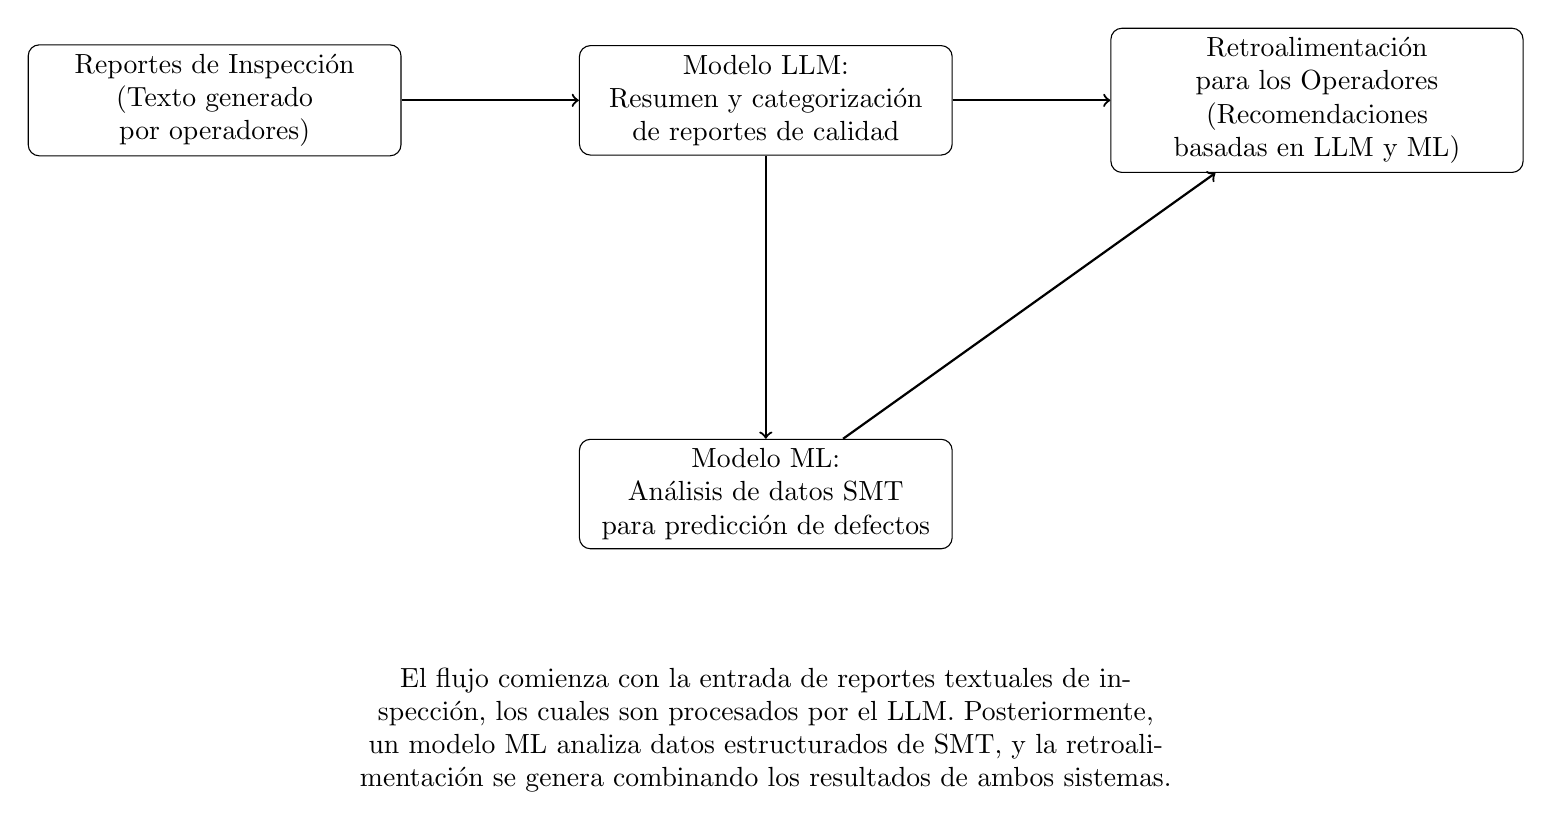
\begin{tikzpicture}[node distance=3cm]
    % Nodos principales
    \node (input1) [draw, rectangle, text width=4.5cm, align=center, rounded corners] 
    {Reportes de Inspección \\ (Texto generado por operadores)};
    
    \node (llm) [right of=input1, xshift=4cm, draw, rectangle, text width=4.5cm, align=center, rounded corners] 
    {Modelo LLM: \\ Resumen y categorización de reportes de calidad};

    \node (ml) [below of=llm, yshift=-2cm, draw, rectangle, text width=4.5cm, align=center, rounded corners] 
    {Modelo ML: \\ Análisis de datos SMT para predicción de defectos};

    \node (output) [right of=llm, xshift=4cm, draw, rectangle, text width=5cm, align=center, rounded corners] 
    {Retroalimentación para los Operadores \\ (Recomendaciones basadas en LLM y ML)};
    
    % Flechas de conexión
    \draw[->, thick] (input1) -- (llm);
    \draw[->, thick] (llm) -- (output);
    \draw[->, thick] (llm) -- (ml);
    \draw[->, thick] (ml) -- (output);

    % Descripción debajo del diagrama
    \node (explanation) [below of=ml, node distance=3cm, text width=12cm, align=center] 
    {El flujo comienza con la entrada de reportes textuales de inspección, los cuales son procesados por el LLM. Posteriormente, un modelo ML analiza datos estructurados de SMT, y la retroalimentación se genera combinando los resultados de ambos sistemas.};
\end{tikzpicture}
\caption{Diagrama del Flujo de Trabajo del Proyecto}
\end{figure}

\subsubsection{Fase 1: Implementación de LLM para la Interpretación de Reportes de Inspección}

En la Fase 1, se utiliza un \textbf{Modelo de Lenguaje Extenso (LLM)} como GPT-4 para procesar los reportes textuales generados por los operadores. Estos reportes suelen contener descripciones detalladas de defectos observados, comentarios sobre posibles causas y acciones recomendadas.

\textbf{Objetivos:}
\begin{itemize}
    \item Procesar grandes volúmenes de texto en tiempo real.
    \item Generar resúmenes automáticos que agrupen defectos comunes y los prioricen según su gravedad.
    \item Facilitar la comunicación entre operadores y supervisores.
\end{itemize}

\textbf{Beneficios:}
\begin{itemize}
    \item Reducción de la carga laboral para supervisores.
    \item Mejora en la comunicación entre operadores y supervisores.
\end{itemize}

\subsubsection{Fase 2: Implementación de ML para el Análisis de Datos SMT}

En la Fase 2, se entrenará un modelo de \textbf{Machine Learning (ML)} utilizando datos estructurados generados por la línea SMT. Estos datos incluyen tiempos de ciclo, temperatura de soldadura y tasa de defectos.

\textbf{Objetivos:}
\begin{itemize}
    \item Predecir defectos antes de que se presenten.
    \item Optimizar los procesos de inspección.
\end{itemize}

\textbf{Beneficios:}
\begin{itemize}
    \item Reducción de retrabajos y scrap.
    \item Aumento en la precisión de las inspecciones.
\end{itemize}

\subsubsection{Fase 3: Integración de LLM y ML para una Retroalimentación Integral}

La integración de los modelos \textbf{LLM} y \textbf{ML} permitirá la creación de un sistema de retroalimentación continua donde tanto los datos textuales como los estructurados se utilicen en conjunto para optimizar las inspecciones y predicciones de defectos.

\textbf{Objetivos:}
\begin{itemize}
    \item Combinar la capacidad del LLM para procesar texto no estructurado con la precisión del ML.
    \item Ofrecer recomendaciones en tiempo real a los operadores.
\end{itemize}

\textbf{Beneficios:}
\begin{itemize}
    \item Optimización en la toma de decisiones.
    \item Mejora continua en el proceso de inspección.
\end{itemize}

\subsection{Costo de la Transición de LLM a ML}

\begin{itemize}
    \item \textbf{LLM:} Bajo costo inicial, ideal para el procesamiento de texto no estructurado, pero limitado en precisión para manejar datos numéricos.
    \item \textbf{ML:} Mayor costo inicial debido a la infraestructura y personal especializado, pero con mayor precisión en predicciones basadas en datos estructurados.
\end{itemize}



\subsubsection{Tabla de Comparación de Fases y Resultados Esperados}

\begin{table}[htbp]
\centering
\caption{Comparación de Resultados Esperados por Fase}
\begin{tabularx}{\textwidth}{|X|X|X|}
\hline
\textbf{Fase} & \textbf{Tecnología Utilizada} & \textbf{Resultados Esperados} \\
\hline
\textbf{Fase 1} & LLM para procesamiento de texto & Reducción del tiempo de análisis de reportes, mejora en la comunicación operador-supervisor. \\
\hline
\textbf{Fase 2} & ML para análisis de datos SMT & Predicción temprana de defectos, reducción de scrap y retrabajos. \\
\hline
\textbf{Fase 3} & Integración LLM + ML & Optimización de la retroalimentación y mejora en la toma de decisiones en tiempo real. \\
\hline
\end{tabularx}
\end{table}
\subsubsection*{Tabla 1: Datos de SMT Antes de la Implementación de IA}

\begin{table}[htbp]
\centering
\caption{Datos de Colocación de Componentes SMT Antes de Implementar IA}
\label{tab:antes-ia-smt}
\begin{tabularx}{\textwidth}{|X|X|X|X|}
\hline
\textbf{Máquina SMT} & \textbf{Cantidad de Componentes Colocados} & \textbf{Tiempo de Ciclo (ms)} & \textbf{Defectos Detectados Manualmente} \\
\hline
SMT Línea 1 & 1500 & 200 & N/A \\
\hline
SMT Línea 2 & 1400 & 195 & N/A \\
\hline
SMT Línea 3 & 1600 & 210 & N/A \\
\hline
SMT Línea 4 & 1550 & 205 & N/A \\
\hline
SMT Línea 5 & 1450 & 190 & N/A \\
\hline
\end{tabularx}
\end{table}

\subsubsection*{Tabla 2: Datos de SMT Después de Implementar IA}

\begin{table}[htbp]
\centering
\caption{Datos de Colocación de Componentes SMT Después de Implementar IA}
\label{tab:despues-ia-smt}
\begin{tabularx}{\textwidth}{|X|X|X|X|X|}
\hline
\textbf{Máquina SMT} & \textbf{Cantidad de Componentes Colocados} & \textbf{Tiempo de Ciclo (ms)} & \textbf{Defectos Detectados} & \textbf{Análisis de Causas} \\
\hline
SMT Línea 1 & 1500 & 200 & 3 & Mala colocación de componentes por desviación de la boquilla \\
\hline
SMT Línea 2 & 1400 & 195 & 1 & Sobrecarga de pasta en PCB \\
\hline
SMT Línea 3 & 1600 & 210 & 0 & Sin anomalías \\
\hline
SMT Línea 4 & 1550 & 205 & 2 & Desplazamiento del componente debido a vibraciones \\
\hline
SMT Línea 5 & 1450 & 190 & 1 & Problema en el alineamiento óptico \\
\hline
\end{tabularx}
\end{table}

\subsubsection{Referencias}
\begin{itemize}
    \item Brown, T., Mann, B., Ryder, N., et al. (2020). \textit{Language Models are Few-Shot Learners}. arXiv preprint arXiv:2005.14165.
    \item Goodfellow, I., Bengio, Y., & Courville, A. (2016). \textit{Deep Learning}. MIT Press.
    \item Kingma, D. P., & Welling, M. (2014). \textit{Auto-Encoding Variational Bayes}. arXiv preprint arXiv:1312.6114.
\end{itemize}

\subsection{Optimización del Proceso en la Industria del Hierro y el Acero con Modelos LLM y ML}

\subsubsection{Contexto y Descripción del Problema}

En la industria del \textbf{hierro y el acero}, uno de los mayores desafíos es la eficiencia operativa en los procesos de fundición, laminación y tratamiento térmico. Actualmente, estos procesos generan grandes cantidades de datos, incluyendo registros (\textit{logs}) de las máquinas, como temperaturas, presiones y tiempos de ciclo. Sin embargo, estos logs no son fácilmente procesables por los operarios, lo que retrasa la detección de problemas y reduce la eficiencia general de la producción.

Para mejorar este proceso, se propone un sistema que utilice un \textbf{Modelo de Lenguaje Extenso (LLM)} para analizar y categorizar los logs generados por las máquinas, combinado con un \textbf{Modelo de Machine Learning (ML)} que permita predecir fallos en los equipos basados en datos estructurados. De este modo, la empresa podrá obtener alertas tempranas sobre problemas de operación y mejorar la calidad y productividad.

\subsection{Objetivos del Proyecto}

El proyecto piloto tiene como objetivo mejorar la eficiencia operativa y la calidad del acero mediante la implementación de IA, tanto para el análisis de logs (datos textuales) como para la predicción de fallos en equipos basados en datos estructurados. 

Las fases del proyecto son las siguientes:

\begin{itemize}
    \item \textbf{Fase 1 (LLM):} Utilizar un modelo LLM para analizar y categorizar los logs de las máquinas, identificando patrones o anomalías que indiquen problemas operativos.
    \item \textbf{Fase 2 (ML):} Entrenar un modelo de ML para predecir fallos en equipos basados en datos estructurados, como la temperatura y presión de los hornos, y la velocidad de las laminadoras.
    \item \textbf{Fase 3:} Integrar ambos modelos (LLM y ML) para generar recomendaciones en tiempo real, ayudando a los operadores a optimizar la producción y evitar fallos no planificados.
\end{itemize}

\section{Flujo de Trabajo del Proyecto}

\begin{figure}[htbp]
\centering
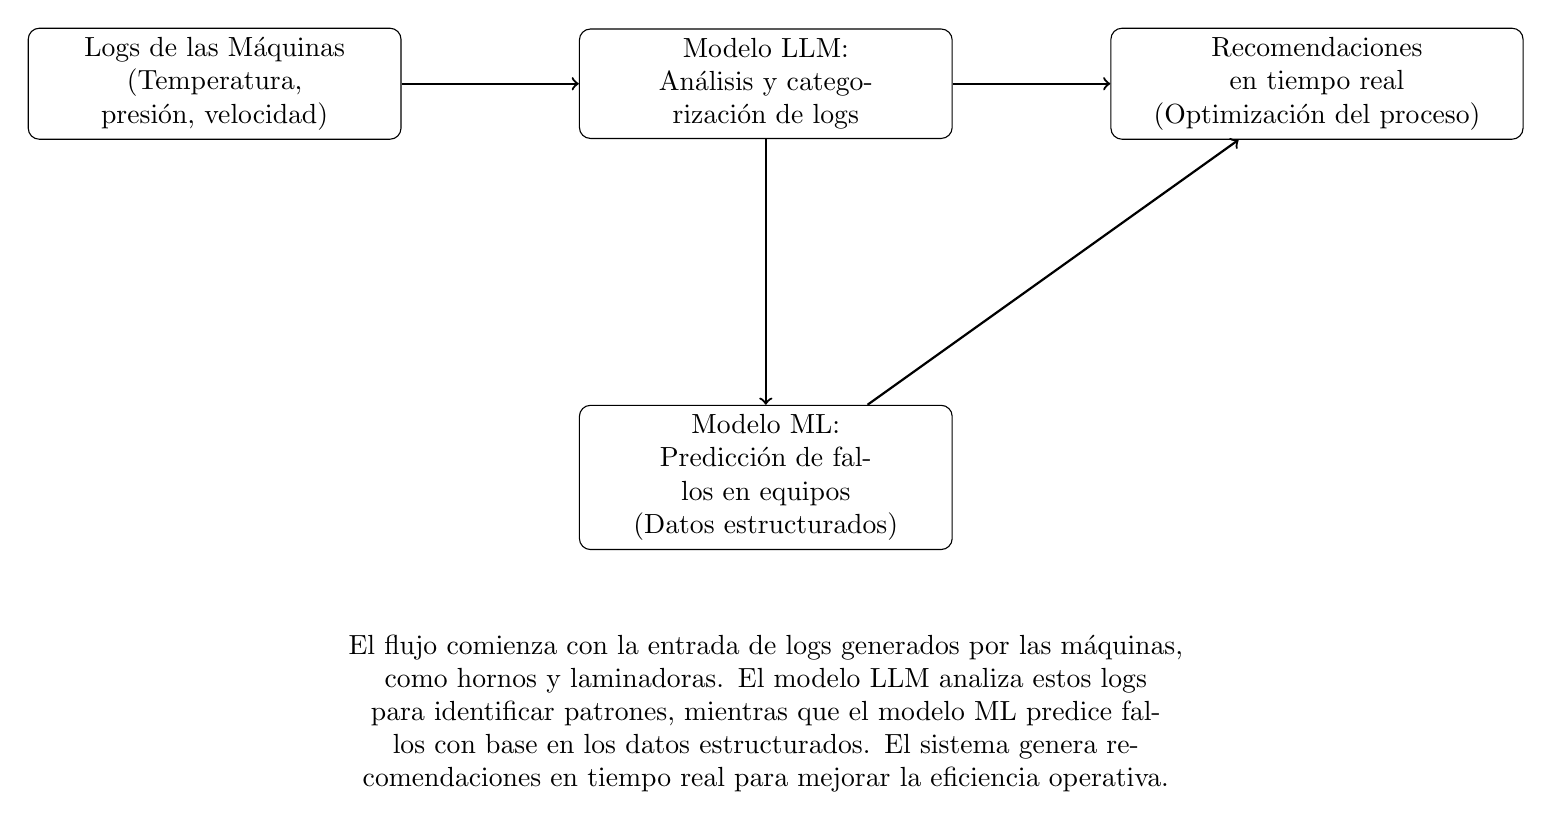
\begin{tikzpicture}[node distance=3cm]
    % Nodos principales
    \node (input1) [draw, rectangle, text width=4.5cm, align=center, rounded corners] 
    {Logs de las Máquinas \\ (Temperatura, presión, velocidad)};
    
    \node (llm) [right of=input1, xshift=4cm, draw, rectangle, text width=4.5cm, align=center, rounded corners] 
    {Modelo LLM: \\ Análisis y categorización de logs};

    \node (ml) [below of=llm, yshift=-2cm, draw, rectangle, text width=4.5cm, align=center, rounded corners] 
    {Modelo ML: \\ Predicción de fallos en equipos \\ (Datos estructurados)};
    
    \node (output) [right of=llm, xshift=4cm, draw, rectangle, text width=5cm, align=center, rounded corners] 
    {Recomendaciones en tiempo real \\ (Optimización del proceso)};

    % Flechas de conexión
    \draw[->, thick] (input1) -- (llm);
    \draw[->, thick] (llm) -- (output);
    \draw[->, thick] (llm) -- (ml);
    \draw[->, thick] (ml) -- (output);

    % Descripción debajo del diagrama
    \node (explanation) [below of=ml, node distance=3cm, text width=12cm, align=center] 
    {El flujo comienza con la entrada de logs generados por las máquinas, como hornos y laminadoras. El modelo LLM analiza estos logs para identificar patrones, mientras que el modelo ML predice fallos con base en los datos estructurados. El sistema genera recomendaciones en tiempo real para mejorar la eficiencia operativa.};
\end{tikzpicture}
\caption{Diagrama del Flujo de Trabajo del Proyecto}
\end{figure}

\subsubsection{Fase 1: Implementación de LLM para Análisis de Logs}

Durante la Fase 1, se implementará un \textbf{Modelo de Lenguaje Extenso (LLM)} para procesar los logs generados por las máquinas en la planta de acero. Estos logs contienen información clave sobre la operación de los hornos de fundición y las laminadoras, incluyendo temperaturas, presiones y tiempos de ciclo.

El modelo LLM se utilizará para:

\begin{itemize}
    \item Identificar patrones anómalos en los logs que puedan estar relacionados con problemas de operación.
    \item Categorizar los logs según los problemas que afectan la eficiencia de las máquinas.
    \item Generar alertas cuando se detecten patrones que indiquen posibles fallos futuros.
\end{itemize}

\textbf{Beneficios:}
\begin{itemize}
    \item Reducción del tiempo necesario para identificar problemas operativos graves en las máquinas.
    \item Mejor categorización de los logs, lo que facilita a los operadores y supervisores tomar decisiones informadas.
    \item Prevención de fallos antes de que afecten de manera significativa a la producción.
\end{itemize}

\subsubsection{Fase 2: Implementación de ML para Análisis de Datos Estructurados}

En la Fase 2, se entrenará un modelo de \textbf{Machine Learning (ML)} utilizando datos estructurados, como la temperatura de los hornos, la presión interna de los equipos y las velocidades de las laminadoras. El objetivo es predecir posibles fallos antes de que ocurran, permitiendo a la planta realizar mantenimientos preventivos de manera proactiva.

Los datos serán recolectados a través de sensores instalados en las máquinas, y el modelo se entrenará utilizando técnicas de regresión y clasificación, optimizando la precisión del modelo para detectar patrones anómalos.

\textbf{Beneficios:}
\begin{itemize}
    \item Predicción precisa de fallos mecánicos, reduciendo el tiempo de inactividad no planificado.
    \item Optimización de los parámetros de operación (temperatura, velocidad) para maximizar la calidad del acero producido.
\end{itemize}

\subsubsection{Fase 3: Integración de LLM y ML para la Retroalimentación Continua}

La Fase 3 consistirá en la integración de los modelos \textbf{LLM} y \textbf{ML} en un sistema único de retroalimentación que proporcione recomendaciones en tiempo real a los operadores de planta. El sistema utilizará los logs analizados por el LLM y los datos estructurados procesados por el ML para ofrecer ajustes operativos en los parámetros de los hornos y laminadoras.

\textbf{Objetivos:}
\begin{itemize}
    \item Proporcionar recomendaciones automáticas a los operadores sobre ajustes de parámetros operativos para evitar fallos.
    \item Mejorar la calidad y consistencia del acero producido mediante el ajuste automático de la temperatura y velocidad de las máquinas.
\end{itemize}

\textbf{Beneficios:}
\begin{itemize}
    \item Mejora de la eficiencia operativa al optimizar continuamente los parámetros de operación.
    \item Reducción en la cantidad de desperdicio de material y mejora en la calidad del producto final.
\end{itemize}

\subsection{Costo de la Transición de LLM a ML}

La transición de LLM a ML en este proyecto implica un análisis de costo-beneficio, donde:

\begin{itemize}
    \item \textbf{LLM:} Es de bajo costo inicial, ya que es rápido de implementar y permite el análisis de logs textuales sin la necesidad de una infraestructura compleja. Es ideal para la fase de identificación temprana de patrones en los datos no estructurados.
    \item \textbf{ML:} Requiere una mayor inversión inicial, tanto en infraestructura como en capacitación, ya que involucra el entrenamiento de modelos basados en grandes volúmenes de datos estructurados (como sensores de temperatura y presión). Sin embargo, a largo plazo ofrece una mayor precisión en la predicción de fallos.
\end{itemize}


\section{Tabla de Resumen del Proyecto}

\begin{table}[htbp]
\centering
\caption{Fases del Proyecto y Beneficios}
\label{tab:resumen-proyecto}
\begin{tabularx}{\textwidth}{|X|X|X|}
\hline
\textbf{Fase} & \textbf{Objetivo} & \textbf{Beneficios} \\
\hline
\textbf{Fase 1} & Implementación de LLM para análisis de logs & Identificación temprana de problemas operativos, mejor categorización de logs \\
\hline
\textbf{Fase 2} & Implementación de ML para análisis de datos estructurados & Predicción de fallos, mantenimiento preventivo, mejora de la eficiencia operativa \\
\hline
\textbf{Fase 3} & Integración de LLM y ML & Retroalimentación en tiempo real, aumento de la eficiencia y mejora en la calidad del producto final \\
\hline
\end{tabularx}
\end{table}

\subsubsection{Tabla 1: Datos de Entrada Antes de la Implementación de IA}

\begin{table}[htbp]
\centering
\caption{Datos de Logs y Sensores Antes de Implementar IA}
\label{tab:antes-ia}
\begin{tabularx}{\textwidth}{|X|X|X|X|}
\hline
\textbf{Máquina} & \textbf{Temperatura (°C)} & \textbf{Presión (Pa)} & \textbf{Velocidad (RPM)} \\
\hline
Horno 1 & 1400 & 100000 & N/A \\
\hline
Horno 2 & 1350 & 95000 & N/A \\
\hline
Laminadora 1 & N/A & N/A & 500 \\
\hline
Laminadora 2 & N/A & N/A & 450 \\
\hline
Horno 3 & 1450 & 105000 & N/A \\
\hline
\end{tabularx}
\end{table}

\section*{Tabla 2: Datos de Entrada Después de Implementar IA}

\begin{table}[htbp]
\centering
\caption{Datos de Logs y Sensores Después de Implementar IA}
\label{tab:despues-ia}
\begin{tabularx}{\textwidth}{|X|X|X|X|X|}
\hline
\textbf{Máquina} & \textbf{Temperatura (°C)} & \textbf{Presión (Pa)} & \textbf{Velocidad (RPM)} & \textbf{Anomalías Detectadas} \\
\hline
Horno 1 & 1400 & 100000 & N/A & No \\
\hline
Horno 2 & 1350 & 95000 & N/A & No \\
\hline
Laminadora 1 & N/A & N/A & 500 & Sí (Variación) \\
\hline
Laminadora 2 & N/A & N/A & 450 & No \\
\hline
Horno 3 & 1450 & 105000 & N/A & Sí (Presión Alta) \\
\hline
\end{tabularx}
\end{table}






\section{Proyectos con el de LLMs(ChatGPT o Gemini)}

\section{Proyecto: Automatización Inteligente de Captura de Facturas}\label{sec:automatizacion-facturas}

\subsection{Eliminando Errores y Agilizando Procesos con IA}

\textbf{Problema Actual:}

En la mayoría de las maquiladoras en Ciudad Juárez, el procesamiento manual de facturas sigue siendo una tarea compleja y repetitiva que consume tiempo y recursos humanos. Imagina un equipo de \textbf{30 capturistas} dedicados exclusivamente a la revisión y captura manual de datos de facturas en diferentes formatos, ya sean PDF, imágenes o archivos XML. Este proceso es propenso a errores humanos y puede retrasar la cadena de suministros, afectando la producción y la relación con los proveedores.

El principal reto aquí es que, aunque la tecnología existe para automatizar este proceso, la mayoría de las maquilas siguen operando con métodos tradicionales, lo que genera ineficiencias que se traducen en costos más altos y tiempos de procesamiento más largos. En un entorno tan competitivo como el de las maquiladoras, esto puede significar una desventaja frente a empresas que ya han implementado tecnologías de automatización.

\textbf{Problema Hipotético:}

Una maquila que procesa \textbf{10,000 facturas mensuales} con diferentes formatos necesita optimizar su proceso para mejorar la eficiencia. Con \textbf{AutoFact 4.0}, el uso de \textbf{Large Language Models (LLM)} como \textbf{GPT-4} o \textbf{Gemini} permite a la maquila reducir significativamente el tiempo y los errores asociados al proceso manual. En lugar de tener un equipo de capturistas trabajando largas jornadas, \textbf{AutoFact 4.0} puede procesar la misma cantidad de facturas en cuestión de horas, utilizando su capacidad para leer, comprender y extraer datos de los diferentes formatos de facturas de manera automática.

\subsubsection{Objetivo del Proyecto}

Implementar \textbf{AutoFact 4.0}, un sistema basado en \textbf{LLM}, que automatice la captura y validación de facturas, utilizando reglas predefinidas de aduanas y normativas locales. Este sistema reducirá la necesidad de intervención humana, acelerará el proceso de facturación y garantizará el cumplimiento normativo con la aduana, optimizando la eficiencia y precisión del proceso.

\subsection{Implementación del Proyecto y Comunicación con Modelos LLM}

\textbf{AutoFact 4.0} no es solo un sistema que extrae información de las facturas; es una solución completa que integra \textbf{inteligencia artificial}, \textbf{procesamiento de lenguaje natural (NLP)} y \textbf{sistemas basados en reglas}. Al trabajar con diferentes formatos de archivos, como \textbf{PDFs} y \textbf{XML}, este sistema no solo identifica y extrae datos relevantes, sino que también los valida con base en \textbf{reglas aduaneras preestablecidas}.

\subsubsection{Paso 1: Recepción y Análisis de Facturas}

El primer paso es la recepción de las facturas. Estas llegan en diferentes formatos, ya sean PDF o XML. Aquí entra en juego una etapa clave de la implementación: la capacidad del sistema para \textbf{comunicarse entre diferentes formatos y los LLM}. Esto implica entrenar el modelo para que pueda interpretar estructuras variables de datos en los PDFs, que son generalmente más complejos, y los XML, que siguen un formato más estandarizado.

\begin{itemize}
    \item \textbf{PDFs}: Utilizando técnicas de reconocimiento óptico de caracteres (\textbf{OCR}), \textbf{AutoFact 4.0} convierte el contenido de las facturas en texto legible para el modelo LLM. A partir de ahí, el modelo extrae información clave como el monto total, el nombre del proveedor, la fecha de emisión y los detalles de los productos.
    \item \textbf{XMLs}: A diferencia de los PDFs, los archivos XML ya contienen la estructura de datos organizada, lo que permite a \textbf{AutoFact 4.0} extraer rápidamente los campos relevantes. El reto con los XML es su variabilidad en el formato dependiendo del proveedor, por lo que el sistema debe ser lo suficientemente flexible para adaptarse a estas diferencias.
\end{itemize}

\subsubsection{Paso 2: Validación Basada en Reglas Aduaneras}

Una vez que se extraen los datos, el siguiente paso es la \textbf{validación} de estos contra reglas aduaneras específicas. El sistema puede integrar una serie de \textbf{reglas predefinidas} que aseguran que los datos capturados cumplan con las regulaciones locales y normativas fiscales.

Por ejemplo, si una factura no incluye los datos necesarios del proveedor o los códigos correctos de los productos, \textbf{AutoFact 4.0} alertará al equipo para que se realicen las correcciones correspondientes antes de aprobar la factura.

\subsubsection{Paso 3: Optimización del Proceso y Reportes en Tiempo Real}

Además de procesar y validar las facturas, \textbf{AutoFact 4.0} también puede generar reportes en tiempo real que muestren el estado de cada factura, si ha sido aprobada, si está pendiente de revisión o si presenta alguna anomalía que necesita ser corregida. Este tipo de visibilidad es crucial para agilizar los tiempos de procesamiento y garantizar que no haya demoras que afecten las operaciones.

\subsection{Diagrama del Proceso}

\begin{figure}[H]
    \centering
    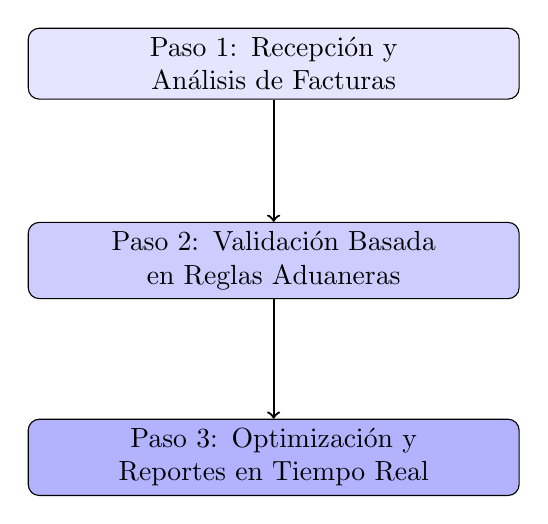
\begin{tikzpicture}
        \node[draw, fill=blue!10, text width=6cm, align=center, rounded corners] (p1) {Paso 1: Recepción y Análisis de Facturas};
        \node[below of=p1, node distance=2.5cm, draw, fill=blue!20, text width=6cm, align=center, rounded corners] (p2) {Paso 2: Validación Basada en Reglas Aduaneras};
        \node[below of=p2, node distance=2.5cm, draw, fill=blue!30, text width=6cm, align=center, rounded corners] (p3) {Paso 3: Optimización y Reportes en Tiempo Real};

        \draw[->, thick] (p1) -- (p2);
        \draw[->, thick] (p2) -- (p3);
    \end{tikzpicture}
    \caption{Diagrama de Proceso de AutoFact 4.0}
\end{figure}
\section{Ejemplo de Factura: Antes y Después del Procesamiento por AutoFact 4.0}

A continuación, se presenta un ejemplo de una factura en formato TXT desordenado antes de ser procesada, y luego el resultado de cómo sería la misma factura después de ser organizada y estructurada por **AutoFact 4.0**.

\begin{table}[H]
\centering
\caption{Comparación de Factura Desordenada y Ordenada por AutoFact 4.0}
\begin{tabularx}{\textwidth}{|X|X|}
\hline
\textbf{Factura Desordenada (Formato TXT/PDF)} & \textbf{Factura Ordenada (AutoFact 4.0)} \\ \hline
\texttt{N\#Factura:  202309123   \hspace{1.2cm}   \\
Proveedor: ACME Corp\\
Articulos:\\
20230912\hspace{0.5cm} Cantidad: 20 \hspace{0.8cm} Producto: Componentes\\
Sub-Total: \$5,000.00\\
IVA: \$800.00 \hspace{2cm}  (16\%)\\
Total:   \$5,800.00   Fecha: 12-09-2023\\
Receptor: Maquila XYZ\\
Direccion:\\ 123 Calle Industrial,\\ Ciudad Juárez, Chihuahua, 32000\\} 
& 
\textbf{N\#Factura:} 202309123 \\
\textbf{Fecha de Emisión:} 12-09-2023 \\
\textbf{Proveedor:} ACME Corp \\
\textbf{Productos:} \\
- \textbf{Descripción:} Componentes \\
- \textbf{Cantidad:} 20 \\
\textbf{Sub-Total:} \$5,000.00 \\
\textbf{IVA (16\%):} \$800.00 \\
\textbf{Total:} \$5,800.00 \\
\textbf{Receptor:} Maquila XYZ \\
\textbf{Dirección de Entrega:} \\
123 Calle Industrial, Ciudad Juárez, Chihuahua, 32000 \\ \hline
\end{tabularx}
\end{table}

\textbf{Descripción del Proceso:}

En la columna izquierda, tenemos un ejemplo de cómo llega la factura en un formato desordenado, ya sea en TXT o PDF, con datos distribuidos de manera inconsistente. Después de que el sistema **AutoFact 4.0** procesa la información, se organiza de forma clara y estructurada, como se muestra en la columna derecha. El sistema es capaz de identificar y extraer automáticamente los campos importantes como el número de factura, el proveedor, la cantidad de productos, el total y otros detalles relevantes, lo que facilita la revisión y validación de la factura.

\subsection{Ventajas de AutoFact 4.0}

\begin{itemize}
    \item \textbf{Reducción de la Intervención Humana}: El número de capturistas se reduce drásticamente. Con AutoFact 4.0, en lugar de 30 capturistas, solo se necesita un equipo pequeño que supervise el sistema.
    \item \textbf{Integración con Normas Aduaneras}: AutoFact 4.0 verifica automáticamente que cada factura cumpla con las normativas vigentes, evitando problemas legales.
    \item \textbf{Mayor Rapidez y Precisión}: Los LLM permiten procesar miles de facturas en minutos con una alta precisión, minimizando errores humanos.
    \item \textbf{Escalabilidad}: El sistema se adapta a un mayor volumen de facturas sin requerir una expansión significativa del equipo humano.
\end{itemize}

\subsection{Consideraciones Técnicas}

La implementación de AutoFact 4.0 requerirá un esfuerzo técnico significativo debido a la integración con los formatos de facturas y la personalización de las reglas aduaneras. Algunos pasos clave incluyen:

\begin{itemize}
    \item Capacitación del equipo de TI en el manejo de LLMs.
    \item Ajuste de las reglas aduaneras para adaptarse a las normativas específicas de cada maquila.
    \item Evaluaciones periódicas para asegurar que el sistema funcione correctamente.
\end{itemize}

\subsection{Comparación Antes y Después de Implementar AutoFact 4.0}

\begin{table}[H]
\centering
\caption{Comparación Antes y Después de Implementar AutoFact 4.0}
\begin{tabular}{|l|c|c|}
\hline
\textbf{Métrica} & \textbf{Antes de AutoFact 4.0} & \textbf{Después de AutoFact 4.0} \\ \hline
Tiempo de procesamiento por factura & 15 minutos por factura & 2 minutos por factura \\ \hline
Errores de captura & 5-10\% & Menos del 1\% \\ \hline
Cantidad de capturistas & 30 capturistas & 5 supervisores \\ \hline
Costo estimado por factura & \$0.10 USD & \$0.02 USD \\ \hline
Facturas procesadas al mes & 10,000 facturas & 10,000 facturas (con posibilidad de escalar) \\ \hline
\end{tabular}
\end{table}

\subsubsection{Costo Estimado del Proyecto}

El costo estimado por factura utilizando \textbf{AutoFact 4.0} se reducirá de \$0.10 USD a \$0.02 USD, lo que representa una reducción significativa de costos. Además, se reducirá el tiempo de procesamiento y se incrementará la precisión de los datos, mejorando la eficiencia general del proceso de captura de facturas en la maquila.


